\documentclass[12pt]{article}

% 导入引言区
\usepackage{array}
\usepackage{amssymb}
\usepackage{amsmath}
\usepackage{ntheorem}
\usepackage{epsf}
\usepackage{color}
\usepackage{xcolor}
\usepackage{graphicx}
\usepackage{epstopdf}
\usepackage{subfigure}
\usepackage{arydshln}
\usepackage{makecell}
\usepackage{mathrsfs}
\usepackage{multirow}
\usepackage{longtable}
\usepackage{threeparttable}
\usepackage{url}
\usepackage{makecell}
\usepackage{booktabs}
\usepackage{listings}
\usepackage{float}
\usepackage{diagbox}
\lstset{numbers=left, %设置行号位置
        numberstyle=\tiny, %设置行号大小
        keywordstyle=\color{blue}, %设置关键字颜色
        commentstyle=\color[cmyk]{1,0,1,0}, %设置注释颜色
        frame=single, %设置边框格式
        escapeinside=``, %逃逸字符(1左面的键)，用于显示中文
        %breaklines, %自动折行
        extendedchars=false, %解决代码跨页时，章节标题，页眉等汉字不显示的问题
        xleftmargin=2em,xrightmargin=2em, aboveskip=1em, %设置边距
        tabsize=4, %设置tab空格数
        showspaces=false %不显示空格
        title=false
}

\usepackage[bookmarks=false]{hyperref}
\hypersetup{hidelinks,
	colorlinks=true,
	allcolors=blue,
	pdfstartview=Fit,
	breaklinks=true}


\usepackage[ruled, linesnumbered]{algorithm2e}
\def\bfm#1{\mbox{\boldmath$#1$}}
\setlength{\arraycolsep}{2pt}
% \def\T{{ \mathrm{\scriptscriptstyle T} }}
\textwidth 165mm
\textheight 220mm
\numberwithin{equation}{section}

% 定义参考文献的格式
\usepackage[style=authoryear, giveninits=true, uniquename=init, backend=biber, maxbibnames=99, minbibnames=3, maxcitenames=2]{biblatex}

% ==========================================
% --- 针对期刊 (Article) 的智能定制 ---
% ==========================================
% 1. 姓名格式调整：去掉名字缩写后面的句号 (H. -> H)
\renewcommand*{\bibinitperiod}{}

% 2. 姓名格式调整：去掉姓和名之间的逗号 (Akaike, H -> Akaike H)
\renewcommand*{\revsdnamepunct}{}

% 3. 卷号调整：强制将期刊的卷号 (Volume) 设置为加粗
\DeclareFieldFormat[article]{volume}{\textbf{#1}}

% 4. 标题调整：去掉文章标题两边的默认双引号
\DeclareFieldFormat[article,inbook,incollection,inproceedings]{title}{#1}

% 5. 期刊前缀调整：去掉默认的 "In: " 字样
\renewbibmacro{in:}{%
  \ifboolexpr{test {\ifentrytype{incollection}} or test {\ifentrytype{inproceedings}}}
    {\printtext{In\space}}
    {}%
}
\DeclareFieldFormat[article]{number}{\mkbibparens{#1}}

% 3. 彻底重写“卷号+期号”的拼接逻辑：去掉它们中间的点，让它们紧紧贴在一起
\renewbibmacro*{volume+number+eid}{%
  \printfield{volume}%
  \printfield{number}% 这里直接跟着期号，不加任何点或空格
  \setunit{\addcomma\space}%
  \printfield{eid}}
\DeclareFieldFormat[article]{pages}{#1}
\DeclareNameAlias{sortname}{family-given}
\renewcommand*{\bibinitdelim}{}
\renewcommand*{\finalnamedelim}{\addspace\&\space}
\renewbibmacro*{name:andothers}{\ifboolexpr{test {\ifnumequal{\value{listcount}}{\value{liststop}}} and test \ifmorenames}{\ifnumgreater{\value{liststop}}{1}{\finalandcomma}{}\printdelim{andothersdelim}\textit{et al.}}{}}
\DeclareFieldFormat{doi}{https://doi.org/#1}
\DeclareFieldFormat{doi}{\url{https://doi.org/#1}}

\renewbibmacro*{addendum+pubstate}{%
  \printfield{addendum}%
  \iffieldundef{pubstate}
    {}
    {\setunit{\addcomma\space}% 强制将前面的标点改为逗号
     \printfield{pubstate}}%
}

% ==========================================
% --- 针对书籍 (Book) 的智能定制 ---
% ==========================================

% 1. 仅针对 book 释放卷号和版本号的默认格式
\DeclareFieldFormat[book]{volume}{#1}
\DeclareFieldFormat[book]{edition}{#1}

% 2. 带有“类型隔离”的安全书名宏
\renewbibmacro*{title}{%
  \ifboolexpr{test {\iffieldundef{title}} and test {\iffieldundef{subtitle}}}
    {}
    {\printtext[title]{%
       \printfield[titlecase]{title}%
       \setunit{\subtitlepunct}%
       \printfield[titlecase]{subtitle}}%
     % --- 核心修正开始：增加类型判断 ---
     \ifentrytype{book}
       {\setunit{\addspace}% 【如果是书籍】加空格，准备拼接括号
        \ifboolexpr{test {\iffieldundef{volume}} and test {\iffieldundef{edition}}}
          {} 
          {\printtext[parens]{% 加上小括号
             \iffieldundef{volume}{}{Vol.\addspace\printfield{volume}}%
             \ifboolexpr{not test {\iffieldundef{volume}} and not test {\iffieldundef{edition}}}
               {\addcomma\space}{}%
             \iffieldundef{edition}{}{\printfield{edition}\addspace Edition}%
           }}%
        \clearfield{volume}% 仅清除书籍的卷号，绝不碰期刊的卷号！
        \clearfield{edition}% 
       }
       {}% 【如果不是书籍】（如期刊Article），什么都不做，安全退出
     % --- 核心修正结束 ---
     \newunit}%
}

% 3. 彻底重写出版社和出版地的排列逻辑 (Publisher, Location)
\renewbibmacro*{publisher+location+date}{%
  \printlist{publisher}% 先打印出版社
  \setunit*{\addcomma\space}% 插入“逗号+空格”
  \printlist{location}% 再打印出版地
  \newunit}

% ==========================================
% --- 针对书籍章节 (Incollection) 的定制 ---
% ==========================================

% 1. 去掉页码前面的 "pp."
\DeclareFieldFormat[incollection]{pages}{#1}

% 2. 将页码强行拼接到所在书名 (booktitle) 后面，并用逗号隔开
\renewbibmacro*{booktitle}{%
  \ifboolexpr{test {\iffieldundef{booktitle}} and test {\iffieldundef{booksubtitle}}}
    {}
    {\printtext[booktitle]{%
       \printfield[titlecase]{booktitle}%
       \setunit{\subtitlepunct}%
       \printfield[titlecase]{booksubtitle}}%
     \iffieldundef{pages}
       {}
       {\setunit{\addcomma\space}% 插入逗号和空格
        \printfield{pages}% 打印页码
        \clearfield{pages}}% 关键：打印完立刻销毁，防止结尾重复打印
    }%
}

% ==========================================
% --- 针对预印本 (Preprint) 的智能定制 ---
% ==========================================
\DeclareFieldFormat[unpublished,inbook,incollection,inproceedings]{title}{#1}

% 导入参考文献库
\addbibresource{ref/refs.bib}

\begin{document}

% 导入定义符号
% 0. Example et al

%\renewcommand{\theequation}{\thesection.\arabic {equation}}
\theoremstyle{plain}
\newtheorem{corollary}{Corollary}[section]
\newtheorem{definition}{Definition}[section]
\newtheorem{example}{Example}[section]
\newtheorem{lemma}{Lemma}%[section]
\newtheorem{property}{Property}[section]
\newtheorem{remark}{Remark}[section]
\newtheorem{theorem}{Theorem}%[section]
\newtheorem{Table}{Table}
\newtheorem{proof}{Proof}
%\renewcommand{\qedsymbol}{}


% 1. Empty-style

\newcommand{\bbB}{{\mathbb{B}}}
\newcommand{\bbC}{{\mathbb{C}}}
\newcommand{\bbD}{{\mathbb{D}}}
\newcommand{\bbE}{{\mathbb{E}}}
\newcommand{\bbI}{{\mathbb{I}}}
\newcommand{\bbJ}{{\mathbb{J}}}
\newcommand{\bbK}{{\mathbb{K}}}
\newcommand{\bbN}{{\mathbb{N}}}
\newcommand{\bbO}{{\mathbb{O}}}
\newcommand{\bbP}{{\mathbb{P}}}
\newcommand{\bbR}{{\mathbb{R}}}
\newcommand{\bbS}{{\mathbb{S}}}
\newcommand{\bbT}{{\mathbb{T}}}
\newcommand{\bbV}{{\mathbb{V}}}
\newcommand{\bbX}{{\mathbb{X}}}
\newcommand{\bbY}{{\mathbb{Y}}}


% 2. Calligraphic

\newcommand{\cA}{{\cal A}}         \newcommand{\dA}[1]{{\cal A}_{#1}}
\newcommand{\cB}{{\cal B}}         \newcommand{\dB}[1]{{\cal B}_{#1}}
\newcommand{\cI}{{\cal I}}
\newcommand{\cJ}{{\cal J}}
\newcommand{\cK}{{\cal K}}
\newcommand{\cN}{{\cal N}}
\newcommand{\cO}{{\cal O}}
\newcommand{\cP}{{\cal P}}
\newcommand{\cS}{{\cal S}}         \newcommand{\dS}[1]{{\cal S}_{#1}}
\newcommand{\cR}{{\cal R}}
\newcommand{\cT}{{\cal T}}
\newcommand{\cU}{{\cal U}}
\newcommand{\cV}{{\cal V}}
\newcommand{\cX}{{\cal X}}
\newcommand{\cY}{{\cal Y}}
\newcommand{\cZ}{{\cal Z}}


% 3. Function

\newcommand{\f}[1]{f_{_{\tiny\rm #1}}}  \newcommand{\hf}[1]{\hat{f}_{#1}}
\newcommand{\tf}[2]{f_{{#1}}^{{#2}}}

\newcommand{\h}[1]{h_{_{\tiny\rm #1}}}
\newcommand{\n}[1]{n_{_{\tiny\rm #1}}}
\newcommand{\q}[2]{q_{_{\tiny\rm #1\!, \, #2}}}
\newcommand{\del}[1]{\delta_{_{\tiny\rm #1}}}
\newcommand{\pii}[2]{\pi_{_{\tiny\rm #1\!, \, #2}}}



\newcommand{\y}[2]{y_{#1}^{\rm #2}}
\newcommand{\yb}[1]{{\bar{y}^{\rm #1}}}
\newcommand{\Y}[1]{Y_{\rm #1}}
\newcommand{\YY}[1]{Y_{\! \mbox{\scriptsize #1}}}
\newcommand{\Two}[2]{{#1}_{_{\textrm{#2}}}}


\newcommand{\no}[2] {   \| #1 \|_{_{#2}}   }
\newcommand{\nor}[3]{\|#1\|_{_{#2}}^{#3}}



\newcommand{\bismall}[2]{(\!\!\begin{array}{c} #1 \\ \vspace*{-0.6cm} \\ #2 \end{array} \!\! )}
\newcommand{\bi}[2]{\Big(\!\!\begin{array}{c} #1 \\ #2 \end{array} \!\!\Big)}
\newcommand{\twoc}[2]{\bigg(\!\!\begin{array}{c} #1 \\ #2  \end{array} \!\!\bigg)}
\newcommand{\twolr}[2]{\left(\!\!\begin{array}{c} #1 \\ #2  \end{array} \!\!\right)}

\newcommand{\twob}[2]{\lbrace {#1 \atop #2} \rbrace}
\newcommand{\twoB}[2]{\bigg\{\!\!\begin{array}{c} #1 \\ #2  \end{array} \!\!\bigg\}}


\newcommand{\fourc}[4]{\bigg(\!\!\begin{array}{cc} #1 & #2 \\ #3 & #4 \end{array} \!\!\bigg)}
\newcommand{\fourlr}[4]{\left(\!\!\begin{array}{cc} #1 & #2 \\ #3 & #4 \end{array} \!\!\right)}
\newcommand{\Cases}[4]{\left\{\!\!\begin{array}{ll} #1, & #2,  \\ [3mm]
                                                    #3, & #4  \end{array} \right. }

\newcommand{\threec}[3]{\left(\!\!\begin{array}{c} #1 \\ #2 \\ #3  \end{array} \!\!\right)}
\newcommand{\threetwo}[6]{\left(\!\!\begin{array}{cc}
#1 & #2 \\
#3 & #4 \\
#5 & #6
\end{array} \!\!\right)}

\newcommand{\threethree}[9]{\left(\!\!\begin{array}{ccc}
#1 & #2 & #3 \\
#4 & #5 & #6 \\
#7 & #8 & #9
\end{array} \!\!\right)}



\newcommand{\sr}[1]{\stackrel{#1}{=}}
\newcommand{\srto}[1]{\stackrel{\rm #1}{\to}}
\newcommand{\sle}[1]{\stackrel{#1}{\le}}
\newcommand{\sgr}[1]{\stackrel{#1}{\ge}}
\newcommand{\sge}[1]{\stackrel{#1}{\ge}}
\newcommand{\mc}[1]{\multicolumn{1}{c}{#1}}
\newcommand{\MC}[3]{\multicolumn{#1}{#2}{#3}}
\newcommand{\MR}[3]{\multirow{#1}{#2}{#3}}
\newcommand{\TC}[4]{\contentsline {#1}{\numberline {#2}#3}{#4}}
\newcommand{\LIST}[3]{\contentsline {section}{\numberline {\hspace*{-0.5cm}#1}#2}{#3}}


\newcommand{\Hpi}[1]{\hat{\pi}_{_{\tiny\rm #1}}}
\newcommand{\titem}[1]{\vspace*{-0.15cm}\item[{\rm #1} ]\hspace*{0.1cm}}
\newcommand{\ub}[1]{\underline{\bf #1}}
\newcommand{\RED}[1]{{\color{red} #1}}      \newcommand{\redbf}[1]{{\color{red} \bf #1}}
\newcommand{\GREEN}[1]{{\color{green} #1}}
\newcommand{\BLUE}[1]{{\color{blue} #1}}


\newcommand{\two}[2]{{#1}_{_{\tiny\rm #2}}}
\newcommand{\three}[3]{{#1}_{_{#2, \tiny\rm #3}}}

\newcommand{\threev}[3]{\left(\!\!\begin{array}{c} #1 \\   #2 \\   #3 \end{array} \!\!\right)}

\newcommand{\at}[1]{a^{(t)}_{#1}}
\newcommand{\bt}[1]{b^{(t)}_{#1}}
\newcommand{\ct}[1]{c^{(t)}_{#1}}       \newcommand{\Ct}[1]{C^{(t)}_{#1}}
\newcommand{\dt}[1]{d^{(t)}_{#1}}
\newcommand{\gt}[1]{g^{(t)}_{#1}}
\newcommand{\pt}[1]{p^{(t)}_{#1}}  \newcommand{\ibpt}[1]{\ibp^{(t)}_{#1}}
\newcommand{\rt}[1]{r^{(t)}_{#1}}
\newcommand{\st}[1]{s^{(t)}_{#1}}


% 4. bold 0 & 1

\newcommand{\0}{{\bf 0}\!\!\!{\bf 0}}
\newcommand{\1}{{\bf 1}\!\!\!{\bf 1}}        \def\b1{{\bf 1\!\!\!1}}  % Letter + number
\newcommand{\2}{{\bf 2}\!\!\!{\bf 2}}        \def\b2{{\bf 2\!\!\!2}}  % Letter + number


% 5. bold English Letter

% 5.1    lowercase
\newcommand{\ba}{{\bf a}}
\newcommand{\bb}{{\bf b}}
\newcommand{\bd}{{\bf d}}
\newcommand{\bn}{{\bf n}}
\newcommand{\bm}{{\bf m}}
\newcommand{\bp}{{\bf p}}
\newcommand{\bq}{{\bf q}}
\newcommand{\br}{{\bf r}}
\newcommand{\bs}{{\bf s}}
%\newcommand{\bt}{{\bf t}}
\newcommand{\bu}{{\bf u}}
\newcommand{\bv}{{\bf v}}
\newcommand{\bw}{{\bf w}}
\newcommand{\bx}{{\bf x}}
\newcommand{\by}{{\bf y}}
\newcommand{\bz}{{\bf z}}


% 5.2    uppercase
\newcommand{\bA}{{\bf A}}
\newcommand{\bB}{{\bf B}}
\newcommand{\bC}{{\bf C}}
\newcommand{\bD}{{\bf D}}
\newcommand{\bG}{{\bf G}}
\newcommand{\bH}{{\bf H}}
\newcommand{\bI}{{\bf I}}
\newcommand{\bJ}{{\bf J}}
\newcommand{\bL}{{\bf L}}
\newcommand{\bM}{{\bf M}}
\newcommand{\bO}{{\bf O}}
\newcommand{\bP}{{\bf P}}
\newcommand{\bQ}{{\bf Q}}
\newcommand{\bR}{{\bf R}}
\newcommand{\bS}{{\bf S}}
\newcommand{\bT}{{\bf T}}
\newcommand{\bU}{{\bf U}}
\newcommand{\bV}{{\bf V}}
\newcommand{\bW}{{\bf W}}
\newcommand{\bX}{{\bf X}}
\newcommand{\bY}{{\bf Y}}
\newcommand{\bZ}{{\bf Z}}


% 5.3 italic English Letter

\newcommand{\iba}{{\boldsymbol{a}}}    \newcommand{\ibA}{{\boldsymbol{A}}}
\newcommand{\ibb}{{\boldsymbol{b}}}    \newcommand{\ibB}{{\boldsymbol{B}}}
                                       \newcommand{\ibC}{{\boldsymbol{C}}}
                                       \newcommand{\ibD}{{\boldsymbol{D}}}

\newcommand{\ibh}{{\boldsymbol{h}}}    \newcommand{\ibH}{{\boldsymbol{H}}}

\newcommand{\ibI}{{\boldsymbol{I}}}
\newcommand{\ibJ}{{\boldsymbol{J}}}
\newcommand{\ibla}{{\boldsymbol{\lambda}}}
\newcommand{\ibe}{{\bfm e}}
\newcommand{\ibm}{{\bfm m}}
\newcommand{\ibn}{{\bfm n}}             \newcommand{\ibN}{{\boldsymbol{N}}}

\newcommand{\ibp}{{\boldsymbol{p}}}     \newcommand{\ibP}{{\boldsymbol{P}}}
\newcommand{\ibr}{{\boldsymbol{r}}}
\newcommand{\ibs}{{\boldsymbol{s}}}
\newcommand{\ibt}{{\bfm t}}
\newcommand{\ibu}{{\boldsymbol{u}}}
\newcommand{\ibv}{{\boldsymbol{v}}}
\newcommand{\ibw}{{\boldsymbol{w}}}
\newcommand{\ibx}{{\boldsymbol{x}}}
\newcommand{\ibxizga}{\ibx_i, \ibz_{(i)}, \bga}
\newcommand{\ibxizgat}{\ibx_i, \ibz_{(i)}, \bga^{(t)}}

\newcommand{\ibX}{{\boldsymbol{X}}}
\newcommand{\iby}{{\boldsymbol{y}}}     \newcommand{\ibY}{{\boldsymbol{Y}}}
\newcommand{\ibz}{{\boldsymbol{z}}} \newcommand{\ibzt}{\ibz^{(t)}}
\newcommand{\ibzi}{\ibz_{(i)}}
\newcommand{\ibziT}{\ibz_{(i)}^{\T}}

\newcommand{\ibZ}{{\boldsymbol{Z}}}
\newcommand{\ibT}{{\boldsymbol{T}}}
\newcommand{\ibW}{{\boldsymbol{W}}}

% 6. hat,  tilde,  bar

% 6.1    hat
\newcommand{\hb}{\hat{b}}   \newcommand{\hbB}{\boldsymbol{\hat{\rm B}}}
\newcommand{\hm}{\hat{m}}
\newcommand{\hp}{\hat{p}}
\newcommand{\hq}{\hat{q}}
\newcommand{\hR}{\hat{R}}



\newcommand{\hbr}{\hat{\br}}


\newcommand{\hth}{\hat{\theta}}   \newcommand{\hTh}{\hat{\Theta}}
\newcommand{\hbth}{\boldsymbol{\hth}}
\newcommand{\hvth}{\hat{\vartheta}}
\newcommand{\hmu}{\hat{\mu}}    \newcommand{\hbmu}{\boldsymbol{\hmu}}
\newcommand{\hsi}{\hat{\sigma}}   \newcommand{\hSi}{\hat{\Sigma}}   \newcommand{\hbSi}{\boldsymbol{\hSi}}
\newcommand{\hal}{\hat{\alpha}}   \newcommand{\hbe}{\hat{\beta}}     \newcommand{\hbbe}{\bfm{\hat \beta}}
\newcommand{\hbal}{\boldsymbol{\hal}}
\newcommand{\hga}{\hat{\gamma}}  \newcommand{\hbga}{\boldsymbol{\hga}}
\newcommand{\hpsi}{\hat{\psi}}
\newcommand{\hxi}{\hat{\xi}}
\newcommand{\hpi}{\hat{\pi}} \newcommand{\hbpi}{\boldsymbol{\hpi}}
\newcommand{\hla}{\hat{\lambda}}  \newcommand{\hbla}{\bfm{{\hat \lambda}}}
\newcommand{\hde}{\hat{\delta}}
\newcommand{\hvp}{\hat{\varphi}}    \newcommand{\hbvp}{\boldsymbol{\hvp}}
\newcommand{\hrho}{\hat{\rho}}
\newcommand{\hbrho}{\boldsymbol{\hrho}}
\newcommand{\hbphi}{\bfm{\hat \phi}}
\newcommand{\hphi}{\hat \phi}

% 6.2    wide hat
\newcommand{\whVar}{\widehat{\mbox{Var}}}
\newcommand{\whse}{\widehat{\mbox{se}}}
\newcommand{\whSe}{\widehat{\mbox{Se}}}
\newcommand{\whPr}{\widehat{\Pr}}

\newcommand{\whbH}{\widehat{\bH}}
\newcommand{\whbS}{\widehat{\bS}}
\newcommand{\whbSi}{\widehat{\bSi}}


% 6.3    tilde


\newcommand{\tp}{\tilde{p}}


\newcommand{\tD}{\tilde{D}}
\newcommand{\tQ}{\tilde{Q}}
\newcommand{\tx}{\tilde{x}}
\newcommand{\ty}{\tilde{y}}

\newcommand{\tth}{\tilde{\theta}}     \newcommand{\tbth}{{\bfm \tth}}
\newcommand{\tpi}{\tilde{\pi}}
\newcommand{\tmu}{\tilde{\mu}}
\newcommand{\tbe}{\tilde{\beta}}
\newcommand{\tga}{\tilde{\gamma}}
\newcommand{\tsi}{\tilde{\sigma}}     \newcommand{\tSi}{\tilde{\Sigma}}
\newcommand{\tpsi}{\tilde{\psi}}
\newcommand{\txi}{\tilde{\xi}}
\newcommand{\tvp}{\tilde{\varphi}}



% 6.4     Bar
\newcommand{\Ba}{\bar{a}}       \newcommand{\Bat}[1]{\Ba_{#1}^{(t)}}
\newcommand{\Bb}{\bar{b}}       \newcommand{\Bbt}[1]{\Bb_{#1}^{(t)}}
\newcommand{\Bd}{\bar{d}}       \newcommand{\Bdt}[1]{\Bd_{#1}^{(t)}}
\newcommand{\Bs}{\bar{s}}       \newcommand{\Bst}[1]{\Bs_{#1}^{(t)}}
\newcommand{\Bt}{\bar{t}}
\newcommand{\Bu}{\bar{u}}
\newcommand{\Bv}{\bar{v}}
\newcommand{\Bw}{\bar{w}}
\newcommand{\Bx}{\bar{x}}
\newcommand{\By}{\bar{y}}       \newcommand{\BY}{\bar{Y}}
\newcommand{\Bz}{\bar{z}}

\newcommand{\Bxi}{\bar{\xi}}
\newcommand{\Bvth}{\bar{\vth}}

\newcommand{\BVar}{\overline{\mbox{Var}}}


% 7. Greek Letter

\newcommand{\al}{\alpha}            \newcommand{\alt}{\alpha^{(t)}}
                                    \newcommand{\altI}{\alpha^{(t+1)}}
\newcommand{\be}{\beta}
\newcommand{\ga}{\gamma}            \newcommand{\Ga}{\Gamma}
\newcommand{\gat}{\gamma^{(t)}}
\newcommand{\de}{\delta}            \newcommand{\De}{\Delta}
\newcommand{\la}{\lambda}           \newcommand{\lat}{\la^{(t)}}
                                    \newcommand{\latI}{\la^{(t+1)}}
\newcommand{\La}{\Lambda}
%\newcommand{\si}{\sigma}            \renewcommand{\Si}{\Sigma} %% tian
%\newcommand{\si}{\sigma}           \newcommand{\Si}{\Sigma}
%\newcommand{\tha}{\theta}            \newcommand{\Th}{\Theta}
\newcommand{\tht}{\theta^{(t)}}
\newcommand{\thx}{\theta_x}         \newcommand{\Thx}{\Theta_x}
\newcommand{\thy}{\theta_y}
\newcommand{\piit}{\pi_i^{(t)}}


\newcommand{\ka}{\kappa}
\newcommand{\om}{\omega}            \newcommand{\Om}{\Omega}

\newcommand{\ve}{\varepsilon}
\newcommand{\vp}{\varphi}
\newcommand{\vr}{\varrho}
\newcommand{\vth}{\vartheta}


% 8. Bold Greek Letter

\newcommand{\bxi}{{\bfm \xi}}              \newcommand{\bet}{{\bfm \eta}}
\newcommand{\bphi}{{\boldsymbol{\phi}}}    \newcommand{\bphit}{\bphi^{(t)}}

\newcommand{\bmu}{{\boldsymbol{\mu}}}      \newcommand{\bnu}{{\boldsymbol{\nu}}}
\newcommand{\bla}{{\boldsymbol{\lambda}}}  \newcommand{\bLa}{{\bfm \Lambda}}
\newcommand{\bSi}{{\bfm \Sigma}}
\newcommand{\bom}{{\bfm \omega}}   \newcommand{\bOm}{{\bfm \Omega}}
\newcommand{\bde}{{\bfm \delta}}   \newcommand{\bDe}{{\bfm \Delta}}
\newcommand{\bth}{{\boldsymbol{\theta}}} \newcommand{\btht}{\bth^{(t)}}
\newcommand{\bTh}{{\boldsymbol{\Theta}}}
\newcommand{\bsi}{{\bfm \sigma}}
\newcommand{\bal}{{\boldsymbol{\alpha}}}
\newcommand{\bbe}{{\boldsymbol{\beta}}}
\newcommand{\brho}{{\boldsymbol{\rho}}}

\newcommand{\bpsi}{{\bfm \psi}}          \newcommand{\bPsi}{{\bfm \Psi}}
\newcommand{\bpi}{{\boldsymbol{\pi}}}    \newcommand{\bpit}{\bpi^{(t)}}
\newcommand{\bga}{{\boldsymbol{\gamma}}} \newcommand{\bgat}{\bga^{(t)}}
\newcommand{\bvp}{{\bfm \varphi}}        \newcommand{\bvpt}{\bvp^{(t)}}

% 9. distribution

\newcommand{\Bernoulli}{\mbox{Bernoulli}}
\newcommand{\Binomial}{\mbox{Binomial}}
%\newcommand{\PBb}{\mbox{PB}_{\rm b}}
\newcommand{\BBB}{\mbox{Bernoulli}_2^{\rm bk}}
\newcommand{\BBinomial}{\mbox{BBinomial}}
\newcommand{\Categorical}{\mbox{Categorical}}
\newcommand{\CP}{\mbox{CP}}
\newcommand{\D}{\mbox{D}}
\newcommand{\Degenerate}{\mbox{Degenerate}}
\newcommand{\DExponential}{\mbox{DExponential}}
\newcommand{\Dirichlet}{\mbox{\rm Dirichlet}}
\newcommand{\DMultinomial}{\mbox{DMultinomial}}
\newcommand{\Exponential}{\mbox{Exponential}}
\newcommand{\FDiscrete}{\mbox{FDiscrete}}
\newcommand{\Finite}{\mbox{Finite}}
\newcommand{\GD}{\mbox{GD}}
\newcommand{\GDirichlet}{\mbox{\rm GDirichlet}}
\newcommand{\GLiouville}{\mbox{GLiouville}}
\newcommand{\GPoisson}{\mbox{GPoisson}}
\newcommand{\GP}{\mbox{GP}}  \newcommand{\GPI}{\GP^{\mbox{\scriptsize{(I)}}}} \newcommand{\GPII}{\GP^{\mbox{\scriptsize{(II)}}}}
\newcommand{\Hgeometric}{\mbox{Hgeometric}}
\newcommand{\HPP}{\mbox{HPP}}
\newcommand{\IBeta}{\mbox{IBeta}}
\newcommand{\Ichi}{\mbox{I}\raisebox{0.5ex}{$\chi$}}
\newcommand{\IGamma}{\mbox{IGamma}}
\newcommand{\IGaussian}{\mbox{IGaussian}}
\newcommand{\IWishart}{\mbox{IWishart}}
\newcommand{\Laplace}{\mbox{Laplace}}
\newcommand{\Liouville}{\mbox{Liouville}}
\newcommand{\Logistic}{\mbox{Logistic}}
\newcommand{\Lognormal}{\mbox{Lognormal}}
\newcommand{\mBeta}{\mbox{Beta}}
\newcommand{\mGamma}{\mbox{Gamma}}
\newcommand{\mGaI}{\mbox{Ga}}

\newcommand{\Multinomial}{\mbox{Multinomial}}
\newcommand{\NBinomial}{\mbox{NBinomial}}
\newcommand{\ND}{\mbox{ND}}
\newcommand{\NDirichlet}{\mbox{NDirichlet}}
\newcommand{\NHPP}{\mbox{NHPP}}
\newcommand{\NIW}{\mbox{NIW}}
\newcommand{\Pareto}{\mbox{Pareto}}
\newcommand{\Poisson}{\mbox{Poisson}}
\newcommand{\TBeta}{\mbox{TBeta}}
\newcommand{\Wishart}{\mbox{Wishart}}
\newcommand{\ZIP}{\mbox{ZIP}}
\newcommand{\ZTP}{\mbox{ZTP}}
\newcommand{\ZAP}{\mbox{ZAP}}
\newcommand{\VZIP}{\mbox{VZIP}}
\newcommand{\ZDP}{\mbox{ZDP}}



%\newcommand{\f}[1]{f_{_{\tiny\rm #1}}}  \newcommand{\hf}[1]{\hat{f}_{#1}}

% 10. mbox -- statistics

\newcommand{\rhor}{\rho^{^{\rm real}}}
\newcommand{\rhof}{\rho^{^{\tiny \rm fit}}}

\newcommand{\AIC}{\mbox{AIC}}
\newcommand{\BIC}{\mbox{BIC}}
\newcommand{\Corr}{\mbox{Corr}} \newcommand{\CorrR}{\Corr^{\small \rm{R}}} \newcommand{\CorrF}{\Corr^{\small \rm{fit}}}
\newcommand{\Cov}{\mbox{Cov}}
\newcommand{\sol}{\mbox{sol}}
\newcommand{\se}{\mbox{se}}

\newcommand{\SE}{\mbox{SE}}
\newcommand{\sgn}{{\rm sgn}}
\newcommand{\tr}{\mbox{$\,$tr$\,$}}
\newcommand{\rank}{\mbox{rank}\,}
\newcommand{\Var}{\mbox{Var}}
\newcommand{\Skew}{\mbox{Skew}}
\newcommand{\MSE}{\mbox{MSE}}
\newcommand{\CV}{\mbox{CV}}
\newcommand{\median}{\mbox{median}}

\newcommand{\logit}{\mbox{logit}}
\newcommand{\diag}{\mbox{diag}}
\newcommand{\data}{\mbox{data}}
\newcommand{\KL}{\mbox{KL}}
\newcommand{\IG}{\mbox{IG}}


\newcommand{\qand}{\quad \mbox{and} \quad}
\newcommand{\qqand}{\quad \qand \quad}
\newcommand{\qas}{\quad \mbox{as} \quad}
\newcommand{\qag}{\quad \mbox{against} \quad}
\newcommand{\qfor}{\quad \mbox{for} \quad}
\newcommand{\qor}{\quad \mbox{or} \quad}
\newcommand{\qve}{\quad \mbox{versus} \quad}
\newcommand{\qwh}{\quad \mbox{where} \quad}
\newcommand{\qwi}{\quad \mbox{with} \quad}
\newcommand{\col}{\mbox{: }}
\newcommand{\RE}{\mbox{RE}}
\newcommand{\yes}{\mbox{yes}}
\newcommand{\No}{\mbox{no}}
\newcommand{\DPP}{\mbox{DPP}}

\newcommand{\rd}{\,\mbox{d}}
%\newcommand{\e}{\mbox{e}}
\newcommand{\w}{\mbox{w}}
\renewcommand{\ge}{\geqslant}
\renewcommand{\le}{\leqslant}
\newcommand{\Zp}{Z\hspace{0.02cm}'}


% 11. Simplification

\newcommand{\I}{{\rm I}}
\newcommand{\II}{I\hspace*{-0.4mm}I}
\newcommand{\III}{I\!I\!I}
\newcommand{\IR}{{I\!\! R}}
\newcommand{\IV}{I$\!$V}
\newcommand{\et}{{\it et al}.}
\newcommand{\Et}{{\it et al}.\,}

\newcommand{\yikH}{y_{ik}^{\rm H}}
\newcommand{\ybH}{\bar{y}^{\rm H}}

% 12. Sign

\newcommand{\sd}{\stackrel{{\rm d}}{=}}
\newcommand{\sdt}{$ {\small $\sd$} $}
\newcommand{\heq}{\;\hat{=}\;}
\newcommand{\teq}{\triangleq}
\newcommand{\iid}{\stackrel{{\rm iid}}{\sim}}
\newcommand{\tiid}{i.i.d.$\hspace*{0.08cm}$}
\newcommand{\ind}{\stackrel{{\rm ind}}{\sim}}
\newcommand{\dsim}{\stackrel{.}{\sim}}
\newcommand{\dis}{\displaystyle}
\newcommand{\tex}{\textstyle}
\newcommand{\cf}{cf.$\hspace*{0.1cm}$}
\newcommand{\trv}{r.v.$\hspace*{0.08cm}$}

\newcommand{\T}{\!\top\!}
\newcommand{\na}{\nabla}
\newcommand{\noi}{\noindent}
\newcommand{\ra}{\rightarrow}
\newcommand{\pr}{\propto}
\newcommand{\eq}{\equiv}
\newcommand{\pa}{\partial}
\newcommand{\ol}{\overline}
\newcommand{\non}{\nonumber}
\newcommand{\ap}{\approx}
\newcommand{\Bot}{\;\bot\;}
\newcommand{\inde}{{\Bot\!\!\!\!\!\!\!\Bot}}
\newcommand{\btu}{\bigtriangleup}


% 13. vskip

\newcommand{\vs}{\vspace*{-0.25cm}}
\newcommand{\vkl}{\vskip 0.10in}
\newcommand{\vkL}{\vskip 0.15in}
\newcommand{\vkU}{\vskip 0.30in}

% 14. environment

\newcommand{\namelistlabel}[1]{\mbox{#1}\hfil}
\newenvironment{namelist}[1]{%
\begin{list}{}
       {\let \makelabel \namelistlabel
        \settowidth{\labelwidth}{#1}
        \setlength{\leftmargin}{1.1\labelwidth}   }
        }{%
\end{list} }


% 15. other
\def\bds{\begin{description} \itemsep=-\parsep \itemindent=-0.7 cm}
\def\eds{\end{description}}
\def\i{\item}

% Liu Yin
%\newcommand{\hphi}{\hat{\phi}}
\newcommand{\tphi}{\tilde{\phi}}
\newcommand{\tla}{\tilde{\lambda}}
\newcommand{\MP}{\mbox{MP}}
\newcommand{\twocc}[2]{\bigg\{\!\!\begin{array}{c} #1 \\ #2  \end{array} \!\!\bigg\}}
\newcommand{\bibx}{{\boldsymbol{\bar{x}}}}
\newcommand{\tbmu}{{\boldsymbol{\tilde{\mu}}}}
\newcommand{\gD}{\mbox{\rm gD}}
\newcommand{\HDirichlet}{\mbox{\rm HDirichlet}}
\newcommand{\hbp}{\bfm {\hat p}}


% Lixunjian

\newcommand{\tal}{\tilde{\al}}
\newcommand{\Bpi}{\bar{\pi}}
\newcommand{\Bal}{\bar{\al}}
\newcommand{\Bbe}{\bar{\be}}
\newcommand{\p}[1]{p_{\rm #1}}
\newcommand{\s}[1]{s_{\rm #1}}
\newcommand{\GA}{\mbox{GA}}
\newcommand{\NR}{\mbox{NR}}
\newcommand{\zed}{\mbox{zeta}}

\newcommand{\Casesthree}[6]
{\left\{\!\!\begin{array}{ll} #1 & #2  \\ [2mm]
                              #3 & #4  \\ [2mm]
                              #5 & #6
\end{array} \right. }

\newcommand{\mif}{\mbox{if } \ }

\newcommand{\tha}{\theta}           \newcommand{\Tha}{\Theta}
\newcommand{\ths}{\theta^*}
\newcommand{\thtI}{\theta^{(t+1)}}

% Zhao Yuanfan

% Paper 1: GeGa

\newcommand{\mpr}{\mbox{Pr}}  % = \Pr
\newcommand{\e}{{\rm e}}
\newcommand{\Kur}{\mbox{Kurt}}
\newcommand{\GeGa}{\mbox{Ge-Ga}(\al,\mu,\bla)}
\newcommand{\IGaGa}{\mbox{IGa-Ga}(\al,\mu, \la)}
\newcommand{\IGauGa}{\mbox{IGau-Ga}(\al, \mu, \la)}
\newcommand{\RIGauGa}{\mbox{RIGau-Ga}(\al, \mu, \la)}
\newcommand{\PaGa}{\mbox{Pa-Ga}(\al, \mu, \la)}
\newcommand{\LN}{\mbox{LN}}
\newcommand{\bthtt}{\bth^{(t+1)}}   \newcommand{\bthtI}{\bth^{(t+1)}}
\newcommand{\bbet}{\bbe^{(t)}}
\newcommand{\bbett}{\bbe^{(t+1)}}   \newcommand{\bbetI}{\bbe^{(t+1)}}
\newcommand{\mut}{\mu^{(t)}}
\newcommand{\mutt}{\mu^{(t+1)}}     \newcommand{\mutI}{\mu^{(t+1)}}
\newcommand{\GIG}{\mbox{GIG}}
\newcommand{\GIGau}{\mbox{GIGau}}
\newcommand{\IGa}{\mbox{IGa}}
\newcommand{\RIG}{\mbox{RIG}}
\newcommand{\RIGau}{\mbox{RIGau}}
\newcommand{\Weibull}{\mbox{Weibull}}
\newcommand{\Se}{\mbox{Se}}
\newcommand{\constant}{\mbox{constant}}

% Paper 2: MVGA
\newcommand{\GeGad}{\mbox{Ge-Ga}_d(\al,\bmu,\bla)}
\newcommand{\IGaGad}{\mbox{IGa-Ga}_d(\al,\bmu, \la)}
\newcommand{\LSGIGauGa}{\mbox{LSGIGau-Ga}_d(\al, \bmu, \la)}
\newcommand{\LNGa}{\mbox{LN-Ga}_d(\al,\bmu,\la)}
\newcommand{\tsf}[1]{\textsf{#1}}

% Paper 3: NP-Ga
\newcommand{\NPGa}{\mbox{NP-Ga}_d(\al, \bmu, \ibp)}
\newcommand{\ibg}{\boldsymbol{g}}   \newcommand{\ibgt}[1]{\ibg_{#1}^{(t)}}
\newcommand{\ptI}[1]{p^{(t+1)}_{#1}}
\newcommand{\bvth}{\boldsymbol{\vth}}
\newcommand{\mcL}{\mathcal{L}}

% Paper 4: NPMN

\newcommand{\GeN}{\mbox{Ge-N}_d(\bmu, \bSi, \bla)}
\newcommand{\Kurt}{\mbox{Kurt}}
\newcommand{\At}[1]{\bA_{#1}^{(t)}}
\newcommand{\bmut}{\bmu^{(t)}}
\newcommand{\bmutI}{\bmu^{(t+1)}}
\newcommand{\bSit}{\bSi^{(t)}}  \newcommand{\bSitI}{\bSi^{(t+1)}}
\newcommand{\bBtI}{\bB^{(t+1)}}
\newcommand{\bgatI}{\bga^{(t+1)}}
\newcommand{\btau}{\boldsymbol{\tau}}

\newcommand{\GaN}{\mbox{Ga-N}_d(\bmu, \bSi, \la)}
\newcommand{\IGaN}{\mbox{IGa-N}_d(\bmu, \bSi, \la)}
\newcommand{\IGauN}{\mbox{IGau-N}_d(\bmu, \bSi, \la)}
\newcommand{\RIGauN}{\mbox{RIGau-N}_d(\bmu, \bSi, \la)}

\newcommand{\NPMN}{\mbox{NPM-N}_d(\bmu, \bSi, \ibp)}
\newcommand{\bvptI}{\bvp^{(t+1)}}
\newcommand{\Loglikelihood}{\textsf{Log-likelihood}}
\newcommand{\Rank}{\textsf{Rank}}
\newcommand{\MAE}{\textsf{MAE}}


\voffset -0.5truecm \hoffset -1.5truecm

% 插入标题、作者信息、摘要和关键词
\begin{flushleft}
{\Large \bf Robust statistical inference for multivariate normal scale mixtures: From parametric frameworks to data--driven models with applications}
\end{flushleft}

\smallskip
\begin{flushleft}
{\bf Yuanfan ZHAO$^{{\rm a}, \dag}$}   \ \  and \ \
{\bf Guo-Liang TIAN$^{{\rm a}, *}$}  \ \

\vkL
{\small \it $^{\rm a}$Department of Statistics and Data Science,
                      Southern University of Science and Technology, \\ Shenzhen 518055, Guangdong Province, P. R. China}

\vkL
{\small  $^{\dag}$Equally contributed} \\
{\small  $^*$Corresponding author's Email: \textsf{tiangl@sustech.edu.cn}} \\
% {\small \textsf{07 July 2026 ZYF}}
\end{flushleft}

\baselineskip 0.30in \vskip 0.05in \noi {\bf Abstract:}

\vkL \noi {\bf Keywords:}   

\baselineskip 0.30in
\setcounter{equation}{0}

% 插入文章正文

\input{data/Section1}
\section{$\!\!\!\!\!\!\!$. General Normal Scale Mixture Framework}\label{zyf.four.sec:GeN}    % Section 2

\subsection{Basic properties of $\GeN$ distribution}\label{zyf.four.sec:GeN.definition}        % Section 2.1

Let a positive \trv $\tau$ follow a general continuous distribution with pdf $f_\tau(\tau | \bla)$, where $\bla = (\la_1, \dots, \la_m)$ is an unknown parameter vector. If a \trv $\ibX = (X_1, \dots, X_d)^\top$ has following SR:
\begin{eqnarray}    \label{zyf.four.2.1}
    \ibX \sd \bmu + \frac{\ibZ}{\sqrt{\tau}}, 
\end{eqnarray}
where $\ibZ = (Z_1, \dots, Z_d)^\top \sim N_d(\0, \bSi)$ and $\ibZ \inde \tau$, then $\ibX$ is said to follow the \textit{general mixture of multivariate normal} (Ge-N$_d$) distribution, denoted by $\ibX \sim \GeN$ or $\mbox{Ge-N}_d(\bth)$ with parameter vector $\bth = \{\bmu, \bSi, \bla\}$. In the SR above, we say $\bmu = (\mu_1, \dots, \mu_d) \in \bbR^d$ is the location parameter and $\bSi = (\sigma_{ij})_{d \times d}$ is the scale parameter matrix. Its joint pdf is
\begin{eqnarray}    \label{zyf.four.2.2}
    \mbox{Ge-N}_d(\ibx | \bth) = \frac{1}{(2\pi)^\frac{d}{2} |\bSi|^\frac{1}{2}} \int_0^\infty h_*(\tau | \ibx, \bth) \rd \tau, \quad \ibx \in \bbR^d,
\end{eqnarray}
where $h_*(\tau | \ibx, \bth) = \tau^\frac{d}{2} f_\tau(\tau | \bla) \exp[-\tau(\ibx - \bmu)^\top \bSi^{-1} (\ibx - \bmu) / 2]$. And the conditional distribution of $\tau | \ibX$ is
\begin{eqnarray}    \label{zyf.four.2.3}
    f_{\tau | \ibX} (\tau | \ibx) \pr \tau^\frac{d}{2} f_\tau(\tau | \bla) \exp\left[ -\frac{\tau}{2} (\ibx - \bmu)^\top \bSi^{-1} (\ibx - \bmu) \right], \quad \tau > 0,
\end{eqnarray}
which can be employed to calculate the conditional expectations of $\tau | (\ibX, \bth)$ in the \textit{expectation--maximization} (EM) and \textit{data augmentation} (DA) algorithm in \S\ref{zyf.four.sec:Bayesian}.

Based on SR (\ref{zyf.four.2.1}), we easily obtain the expectation and covariance matrix of $\ibX$ as
\begin{eqnarray}    \label{zyf.four.2.4}
    E(\ibX) = \bmu \qand \Var(\ibX) = E\left( \tau^{-1} \right) \bSi,
\end{eqnarray}
we also consider its kurtosis in each dimension, that is, 
\begin{eqnarray*}
    \Kurt(X_j) = \frac{E\{[X_j - E(X_j)]^4\}}{[\Var(X_j)]^2} - 3 = 3\left\{ \frac{E\left( \tau^{-2} \right)}{\left[ E\left( \tau^{-1} \right)\right]^2} - 1\right\}, \quad j = 1, \dots, d.
\end{eqnarray*}

\begin{remark}{\rm \textbf{(Selection of mixture variable).} In order to completely eliminate the parameter coupling problem between the covariance matrix and the marginal kurtosis and ensure the identifiability, we impose the inverse expectation of mixture variable $E(\tau^{-1}) = 1$ via the scale transformation property in GIGau family (see more details in \S\ref{zyf.four.sec:Specificcase} and \hyperref[zyf.four.sec:SM]{Supplementary Materials}). \hfill$\|$
}\end{remark}

\subsection{MLEs of parameters via N-EM algorithm}\label{zyf.four.sec:NEM}      % Section 2.2

Suppose that $\{\ibX_i\}_{i=1}^n \iid \GeN$ and $\Y{obs} = \{\ibx_i\}_{i=1}^n$ denote the observed data, where $\ibx_i$ is the realizations of $\ibX_i$, the log-likelihood function of $\bth$ is
\begin{eqnarray}    \label{zyf.four.2.5}
    \ell_*(\bth | \Y{obs}) \sr{(\ref{zyf.four.2.2})} -\frac{nd}{2} \log(2\pi) - \frac{n}{2} \log|\bSi| + \sum_{i=1}^n \log \int_0^\infty h_*(\tau | \ibx_i, \bth) \rd \tau,
\end{eqnarray}
Notice that there is a complex integrals in (\ref{zyf.four.2.5}), therefore, some traditional optimization methods like Newton--Raphson algorithm, Fisher scoring algorithm and \textit{minorization--maximization} (MM, \cite{HL2004}) algorithm are not suitable to use. To solve this integrals, we will adopt the N-EM algorithm (\cite{TL2022}) with the following three steps:
\begin{namelist}{01234567}
\item[\hspace*{-0.08cm} \textsf{N-step}:] By normalizing $h_*(\tau | \ibx_i, \bth)$, we construct a \textit{normalizing density function} (ndf)
	$$
       g_*(\tau | \ibx_i, \bth) \teq \frac{h_*(\tau | \ibx_i, \bth)}{\int_0^\infty h_*(s | \ibx_i, \bth) \rd s}, \quad \tau > 0,
	$$
    so that $g_*(\tau | \ibx_i, \btht)$ is also a density function defined on $\bbR_+$, where $\btht$ denotes the $t$-th approximation of the MLE $\hbth$.

\item[\hspace*{-0.08cm} \textsf{E-step}:] To construct a surrogate function satisfying $Q_*(\bth | \btht) \le \ell_*(\bth | \Y{obs})$ and $Q_*(\btht | \btht)$ $=\ell_*(\btht | \Y{obs})$, we use the Jensen's inequality to obtain
	\begin{eqnarray}   \label{zyf.four.2.6}
        Q_*(\bth | \btht) &=& \ct{*} - \frac{n}{2} \log|\bSi| - \frac{1}{2} \sum_{i=1}^n \at{i*} (\ibx_i - \bmu)^\top \bSi^{-1} (\ibx_i - \bmu) \non \\ [2mm]
        && +\; \sum_{i=1}^n \int_0^\infty \log[f_\tau(\tau | \bla)] \cdot g_*(\tau | \ibx_i, \btht) \rd \tau,
	\end{eqnarray}
    which minorizes $\ell_*(\bth | \Y{obs})$ at $\bth = \btht$, where $\ct{*}$ is a constant free from $\bth$ and
    \begin{eqnarray}    \label{zyf.four.2.7}
        \at{i*} \teq \int_0^\infty \tau \cdot g_*(\tau | \ibx_i, \btht) \rd \tau, \quad i = 1, \dots, n.
    \end{eqnarray}
	
\item[\hspace*{-0.08cm} \textsf{M-step}:] Given $\btht$, by maximizing $Q_*(\bth | \btht)$ with respect to $\bth$, we update $\btht$ by
	$$
	   \bthtt = \arg \max_{\bth\in\bTh} Q_*(\bth | \btht).
	$$
\end{namelist}
Given a pre-specified small positive number $\de_0$, the N-, E- and M-steps are alternately repeated until
$$
    \bigg|\frac{\ell_*(\bthtt | \Y{obs}) - \ell_*(\btht | \Y{obs})}{\ell_*(\btht | \Y{obs})}\bigg| \le \de_0,
$$
then we obtain the MLE $\hbth$ of parameter vector $\bth$. Based on (\ref{zyf.four.2.6}), we take the first derivative of $Q_*(\bth | \btht)$ and solve the following system of equations:
\begin{eqnarray*}
    && \frac{\pa Q_*(\bth | \btht)}{\pa \bmu} = \bSi^{-1} \sum_{i=1}^n \at{i*}(\ibx_i - \bmu) = \0_d, \\ [2mm]
    && \frac{\pa Q_*(\bth | \btht)}{\pa \bSi} = -\frac{n}{2} \bSi^{-1} + \frac{1}{2} \sum_{i=1}^n \at{i*}(\ibx_i - \bmu)(\ibx_i - \bmu)^\top \left( \bSi^{-1} \right)^2 = \0_{d \times d}, \\ [2mm]
    && \frac{\pa Q_*(\bth | \btht)}{\pa \la_k} = \sum_{i=1}^n \log \int_0^\infty \frac{\pa \log[f_\tau(\tau|\bla)]}{\pa \la_k} \cdot g_*(\tau | \ibx_i, \btht) \rd \tau = 0, \qfor k = 1, \dots, m.
\end{eqnarray*}
We obtain the $(t+1)$-th approximation of $\hbth$ as
\begin{eqnarray}    \label{zyf.four.2.8}
    \left\{
    \begin{array}{lll}
        \bmutI &=& \dis \frac{\sum_{i=1}^n \at{i*} \ibx_i}{\sum_{i=1}^n \at{i*}} = \bX \ibpt{*}, \\ [6mm]
        \bSitI &=& \dis \frac{1}{n} \sum_{i=1}^n \at{i*} \left( \ibx_i - \bmutI\right) \left( \ibx_i - \bmutI\right)^\top \\ [6mm]
        &=& \dis \frac{1}{n}\left(\bX - \1_n \bmu^{(t+1)\top} \right)^\top \At{*} \left(\bX - \1_n\bmu^{(t+1)\top} \right), \\ [6mm]
        \latI_k &=& \dis \sol\left\{ s_*(\la_k | \Y{obs}, \btht) = 0 \right\}, \qfor k = 1, \dots, m,
    \end{array}
    \right.
\end{eqnarray}
where $\at{i*}$ is defined by (\ref{zyf.four.2.7}), 
$$
    \pt{i*} \teq \frac{\at{i*}}{\sum_{j=1}^n \at{j*}}, \quad i = 1, \dots, n \quad \ibpt{*} \teq (\pt{1*}, \dots, \pt{n*})^\top,  
$$
$\bX = (\ibx_1, \dots, \ibx_n)^\top$, $\At{*} = \diag(\at{1*}, \dots, \at{n*})$ and the symbol ``$\sol\{s_*(\la_k | \Y{obs}, \btht) = 0\}$'' denotes the unique root of the equation $s_*(\la_k | \Y{obs}, \btht) = 0$ with
$$
    s_*(\la_k | \Y{obs}, \btht) = \sum_{i=1}^n \log \int_0^\infty \frac{\pa \log[f_\tau(\tau|\bla^{(t+1,t)})]}{\pa \la_k} \cdot g_*(\tau | \ibx_i, \btht) \rd \tau,
$$
where $\bla^{(t+1,t)} \teq \left( \latI_1, \dots, \latI_{k-1}, \la_k, \lat_{k+1}, \dots, \lat_m \right)^\top$.

\subsection{Mean regression model for $\GeN$ distribution}       % Section 2.3

From (\ref{zyf.four.2.4}), we know the expectation of Ge-N$_d$ distribution is $\bmu$, therefore, by assuming that $\{\ibX_i\} \ind \mbox{Ge-N}_d(\bmu_i, \bSi, \bla)$ and observed data $\Y{obs} = \{\ibx_i, \ibzi\}_{i=1}^n$, we consider the following mean regression model
\begin{eqnarray}    \label{zyf.four.2.9}
    E(\ibX_i | \ibzi) = \bmu_i = \bB^\top \ibzi, \quad i = 1, \dots, n,
\end{eqnarray}
where $\ibzi = (z_{i1}, \dots, z_{iq})^\top$ is a $q$-dimensional vector of covariates for the $i$-th subject, the matrix of regression coefficients
\begin{eqnarray*}
    \bB = \left(
    \begin{array}{cccc}
        \be_{11} & \be_{12} & \cdots & \be_{1d} \\ 
        \be_{21} & \be_{22} & \cdots & \be_{2d} \\ 
        \vdots   & \vdots   & \ddots & \vdots   \\
        \be_{q1} & \be_{q2} & \cdots & \be_{qd}
    \end{array}
    \right),
\end{eqnarray*}
with $q \times d + d(d + 1) / 2 + m \le n$. Let $\bga = \{ \bB, \bSi, \bla\}$ be the parameter vector, based on (\ref{zyf.four.2.2}) and (\ref{zyf.four.2.9}), the log-likelihood function of $\bga$ is
\begin{eqnarray}    \label{zyf.four.2.10}
    \ell(\bga | \Y{obs}) = -\frac{nd}{2} \log(2\pi) - \frac{n}{2} \log|\bSi| + \sum_{i=1}^n \log \int_0^\infty h(\tau | \ibx_i, \ibzi, \bga) \rd \tau,
\end{eqnarray}
where $h(\tau | \ibx_i, \ibzi, \bga) \teq \tau^\frac{d}{2} f_\tau(\tau|\bla) \exp[-\tau(\ibx - \bB^\top \ibzi)^\top \bSi^{-1} (\ibx - \bB^\top \ibzi) / 2]$. To calculate the MLEs of $\bga$, we utilize the N-EM algorithm again. By computing the ndf
$$
    g(\tau | \ibx_i, \ibzi, \bga) \teq \frac{h(\tau | \ibx_i, \ibzi, \bga)}{\int_0^\infty h(s | \ibx_i, \ibzi, \bga) \rd s}, \quad \tau > 0, 
$$
we construct the surrogate function 
\begin{eqnarray*}
    Q(\bga | \bgat) &=& \ct{} - \frac{n}{2} \log|\bSi| - \frac{1}{2} \sum_{i=1}^n \at{i} \left(\ibx_i - \bB^\top \ibzi \right)^\top \bSi^{-1} \left(\ibx_i - \bB^\top \ibzi \right) \\ [2mm]
    && +\; \sum_{i=1}^n \int_0^\infty \log[f_\tau(\tau | \bla)] \cdot g(\tau | \ibx_i, \ibzi, \bgat) \rd \tau,
\end{eqnarray*}
with constant $\ct{}$ and $\at{i} = \int_0^\infty \tau \cdot g(\tau | \ibx_i, \ibzi, \bgat) \rd \tau$ for $i = 1, \dots, n$.

Finally, we maximize $Q(\bga | \bgat)$ respect to $\bga$ in M-step. By solving the following system of equations:
\begin{eqnarray*}
    && \frac{\pa Q(\bga | \bgat)}{\pa \bB} = \sum_{i=1}^n \at{i} \ibzi (\ibx_i - \bB^\top \ibzi)^\top \bSi^{-1} = \0_{q\times d}, \\ [2mm]
    && \frac{\pa Q(\bga | \bgat)}{\pa \bSi} = -\frac{n}{2} \bSi^{-1} + \frac{1}{2} \sum_{i=1}^n \at{i} \left(\ibx_i - \bB^\top \ibzi \right) \left(\ibx_i - \bB^\top \ibzi \right)^\top \left( \bSi^{-1} \right)^2 = \0_{d \times d}, \\ [2mm]
    && \frac{\pa Q(\bga | \bgat)}{\pa \la_k} = \sum_{i=1}^n \log \int_0^\infty \frac{\pa \log[f_\tau(\tau|\bla)]}{\pa \la_k} \cdot g(\tau | \ibx_i, \ibzi, \bgat) \rd \tau = 0, \qfor k = 1, \dots, m.
\end{eqnarray*}
we obtain the $(t+1)$-th approximation of $\hbga$ as
\begin{eqnarray}    \label{zyf.four.2.11}
    \left\{
    \begin{array}{lll}
        \bBtI &=& \dis \left[ \sum_{i=1}^n \at{i} \ibzi \ibziT \right]^{-1} \left[ \sum_{i=1}^n \at{i} \ibzi \ibx_i^\top \right] = \left(\bZ^\top \At{} \bZ\right)^{-1} \left(\bZ^\top \At{} \bX\right), \\ [6mm]
        \bSitI &=& \dis \frac{1}{n} \sum_{i=1}^n \at{i} \left( \ibx_i - \bB^{(t+1)\top} \ibzi\right) \left( \ibx_i - \bB^{(t+1)\top}\ibzi \right)^\top \\ [6mm]
        &=& \dis \frac{1}{n}\left(\bX - \bZ \bBtI \right)^\top \At{} \left(\bX - \bZ \bBtI \right), \\ [6mm]
        \latI_k &=& \dis \sol\left\{ s(\la_k | \Y{obs}, \bgat) = 0 \right\}, \qfor k = 1, \dots, m,
    \end{array}
    \right.
\end{eqnarray}
where $\bZ = (\ibz_{(1)}, \dots, \ibz_{(n)})^\top$, $\At{} = \diag(\at{1}, \dots, \at{n})$, $\bX = (\ibx_1, \dots, \ibx_n)^\top$ and 
$$
    s(\la_k | \Y{obs}, \bgat) = \sum_{i=1}^n \log \int_0^\infty \frac{\pa \log[f_\tau(\tau|\bla^{(t+1,t)})]}{\pa \la_k} \cdot g(\tau | \ibx_i, \ibzi, \bgat) \rd \tau.
$$

\subsection{Bootstrap CIs of $\bth$}     % Section 2.4

The large--sample method for calculating CIs of parameters has two limitations: (1) The asymptotic CI is not reliable for small to moderate sample sizes; and (2) even though for a large sample size, the range of CI may be beyond its bounds when the true value is close to the bounds. To overcome the two difficulties, this subsection presents the bootstrap method (\cite{Efron1992}) to construct the \textit{bootstrap confidence interval} (BCI) (\cite{Hall1988}, \cite{DR1988}) of $\psi \teq u(\bth)$, where $u(\cdot)$ is an arbitrary function of the parameter vector $\bth$ in the $\mbox{Ge-N}_d(\bth)$ distributions.

Based on the observations $\Y{obs} = \{\ibx_i\}_{i=1}^n$, we can first compute the MLEs $\hbth$ of $\bth$ through the N-EM algorithm (\ref{zyf.four.2.8}) or (\ref{zyf.four.2.11}). Then, we generate a bootstrap sample $\{\ibX_i^*= \ibx_i^*\}_{i=1}^n \iid \mbox{Ge-N}_d(\hbth)$ and compute the bootstrap replication $\hpsi^* = u(\hbth^*)$. Independently repeating this process $G$ times, we obtain $G$ bootstrap replications $\{\hpsi^*(g)\}_{g=1}^G$. Hence, a $100(1-\al)$\% BCI of $\psi$ is $[\hpsi_{\rm L}^*, \  \hpsi_{\rm U}^*]$, where $\hpsi_{\rm L}^*$ and $\hpsi_{\rm U}^*$ are the $(\al/2)G$-th and the $(1-\al/2)G$-th order statistics of $\{\hpsi^*(g)\}_{g=1}^G$.

\subsection{Bayesian method}\label{zyf.four.sec:Bayesian}        % Section 2.5

Assume that $\{\ibX_i\}_{i=1}^n \iid \GeN$ and the observed data $\Y{obs} = \{\ibx_i\}_{i=1}^n$. In this section, we perform the empirical Bayesian inference on parameter $\bvth = \{\bmu, \bSi\}$ (\cite{BT1992}). That is, we will compute the posterior mode and generate the posterior sample via ECM algorithm (\cite{MR1993}) and DA algorithm. After generating the posterior sample, the posterior mean, posterior standard error and Bayesian credit interval can be obtained.

In the empirical Bayesian method, our focus is on the parameter $\bvth$, so $\bla$ will be considered as a constant. Therefore, we replace it by $\hbla$, which can be computed by N-EM algorithm in \S\ref{zyf.four.sec:NEM}. Denote the prior distribution of $\bvth$ be $\pi(\bvth)$ and we regard $\Y{mis} = \{\tau_i\}_{i=1}^n \iid f_\tau(\cdot | \hbla)$ as the missing data. Therefore, we obtain the complete data posterior distribution
\begin{eqnarray}    \label{zyf.four.2.12}
    p(\bvth | \Y{com}) \pr L(\bvth | \Y{com}) \cdot \pi(\bvth), \qwi \Y{com} = \{\Y{obs}, \Y{mis}\}.
\end{eqnarray}
Finding the mode of posterior distribution is equivalent to optimizing the function $p(\bvth | \Y{com})$ to obtain the optimized value $\tilde{\bvth}$. We consider the following two situations: the non-information prior and the conjugate prior distribution.

\subsubsection{The ECM algorithm to calculate posterior mode of $\bvth$}        % Section 2.5.1

If we know little about the parameters before experiment, then we need to consider the following non-information (or diffuse) prior distributions:
\begin{eqnarray}    \label{zyf.four.2.13}
    \pi(\bvth) = |\bSi|^{-\frac{d+1}{2}}
\end{eqnarray}
Combine the equations (\ref{zyf.four.2.12}) and (\ref{zyf.four.2.13}), we obtain the posterior distribution
\begin{eqnarray}    \label{zyf.four.2.14}
    p(\bvth | \Y{com}) \pr |\bSi|^{-\frac{n+d+1}{2}} \exp\left[ -\frac{1}{2}\sum_{i=1}^n \tau_i (\ibx_i - \bmu)^\top \bSi^{-1} (\ibx_i - \bmu) \right]
\end{eqnarray}
The CM-step of ECM algorithm is to compute the posterior mode of the complete data, we obtain
\begin{eqnarray*}
    && \tilde{\bmu} = \frac{\sum_{i=1}^n \tau_i \ibx_i}{\sum_{i=1}^n \tau_i} = \frac{\bX^\top \btau}{\1_d^\top \btau} \qand \\ [2mm]
    && \tilde{\bSi} = \frac{\sum_{i=1}^n \tau_i (\ibx_i - \bmu)(\ibx_i - \bmu)^\top}{n + d + 1} = \frac{(\bX - \1_n \bmu^\top)^\top \bT (\bX - \1_n \bmu^\top)}{n + d + 1},
\end{eqnarray*}
where $\bX = (\ibx_1, \dots, \ibx_n)^\top$, $\btau = (\tau_1, \dots, \tau_n)^\top$, $\bT = \diag(\tau_1, \dots, \tau_n)$. Based on (\ref{zyf.four.2.3}), we can compute the conditional expectation of $\tau_i | \ibX_i$. Then the E-step is to replace $\{\tau_i\}_{i=1}^n$ by their conditional expectations
$$
    E(\tau_i | \Y{obs}, \bvth) = \int_0^\infty \tau \cdot g_*(\tau | \ibx_i, \hbla, \bvth) \rd \tau, \quad i = 1, \dots, n.
$$
And according to the posterior distribution (\ref{zyf.four.2.14}), we obtain
\begin{eqnarray}
    && \bmu | (\Y{com}, \bSi) \sim N_d\left( \frac{\bX^\top \btau}{\1_d^\top \btau}, \frac{\bSi}{\1_d^\top \btau} \right) \qand \label{zyf.four.2.15} \\ [2mm]
    && \bSi | (\Y{com}, \bmu) \sim \IWishart_d\left( (\bX - \1_n \bmu^\top)^\top \bT (\bX - \1_n \bmu^\top), n \right), \label{zyf.four.2.16}
\end{eqnarray}
where $\IWishart_d$ means the inverse Wishart distribution (see more details in Appendix \ref{zyf.four.sec:NIW}).

Then we consider the second situation, when the mean and covariance matrices are unknown, the conjugate prior of the multivariate normal distribution is a \textit{normal inverse Wishart} (NIW) distribution (\cite{LW1992}). Therefore, we consider the following conjugate priors:
\begin{eqnarray}    \label{zyf.four.2.17}
    \bmu | \bSi \sim N_d\left( \bmu_0, \frac{\bSi}{\ka_0} \right) \qand \bSi \sim \IWishart_d(\bLa_0, \nu_0),
\end{eqnarray}
where $\nu_0 > d - 1$. That is, $(\bmu, \bSi) \sim \NIW_d(\bmu_0, \ka_0, \bLa_0, \nu_0)$. According to (\ref{zyf.four.2.12}) and (\ref{zyf.four.2.17}), the complete data posterior distribution can be obtained as
\begin{eqnarray}    \label{zyf.four.2.18}
    p(\bvth | \Y{com}) &\pr& |\bSi|^{-\frac{n + \nu_0 + d + 2}{2}} \exp\left[ -\frac{1}{2} \sum_{i=1}^n \tau_i (\ibx_i - \bmu)^\top \bSi^{-1} (\ibx_i - \bmu) \right. \non \\ [2mm]
    && -\; \frac{1}{2}(\bmu - \bmu_0)^\top \bSi^{-1} (\bmu - \bmu_0) - \frac{1}{2}\tr\left(\bLa_0\bSi^{-1}\right)\bigg].
\end{eqnarray}
Therefore, we compute the posterior mode of complete data
\begin{eqnarray*}
    \tilde{\bmu} &=& \frac{\sum_{i=1}^n \tau_i \ibx_i + \ka_0\bmu_0}{\sum_{i=1}^n \tau_i + \ka_0} = \frac{\bX^\top \btau + \ka_0\bmu_0}{\1_d^\top \btau + \ka_0}, \\ [2mm]
    \tilde{\bSi} &=& \frac{\sum_{i=1}^n \tau_i (\ibx_i - \bmu)(\ibx_i - \bmu)^\top + \bLa_0 + \ka_0(\bmu - \bmu_0)(\bmu - \bmu_0)^\top}{n + \nu_0 + d + 2} \\ [2mm]
    &=& \frac{(\bX - \1_n \bmu^\top)^\top \bT (\bX - \1_n \bmu^\top) + \bLa_0 + \ka_0(\bmu - \bmu_0)(\bmu - \bmu_0)^\top}{n + \nu_0 + d + 2},
\end{eqnarray*}
and replace $\{\tau_i\}_{i=1}^n$ by conditional expectations $E(\tau_i | \Y{obs}, \bvth)$. According to the posterior distribution (\ref{zyf.four.2.18}), we obtain
\begin{eqnarray}
    && \bmu | (\Y{com}, \bSi) \sim N_d\left( \frac{\bX^\top \btau + \ka_0\bmu_0}{\1_d^\top \btau + \ka_0}, \frac{\bSi}{\1_d^\top\btau + \ka_0} \right) \qand \label{zyf.four.2.19} \\ [2mm]
    && \bSi | (\Y{com}, \bmu) \sim \IWishart_d(\bf{\Psi}, n + \nu_0 + 1), \label{zyf.four.2.20}
\end{eqnarray}
where the scale matrix $\bf{\Psi} = (\bX - \1_n \bmu^\top)^\top \bT (\bX - \1_n \bmu^\top) + \bLa_0 + \ka_0(\bmu - \bmu_0)(\bmu - \bmu_0)^\top$.

\subsubsection{DA algorithm with an embedded AR algorithm to generate posterior samples}        % Section 2.5.2

In order to make a complete Bayesian inference of $\bvth$, we need to employ the DA algorithm (\cite{TW1987}) to generate sample that follows the posterior distribution. In the I-step of DA algorithm, we need to generate the missing data $\Y{mis} = \{\tau_i\}_{i=1}^n$ from the conditional distribution (\ref{zyf.four.2.3}). Since the function has no explicitly expression, the \textit{acceptance--rejection} (AR) algorithm is used to achieve this step. We choose the envelope density
$$
    m(\tau_i) = \mGamma\left(\tau_i \;\bigg|\; \frac{d}{2} + 1, \frac{(\ibx_i - \bmu)^\top \bSi^{-1} (\ibx_i - \bmu)}{2}\right)
$$
And we compute the ratio
$$
    \frac{f_{\tau_i|\ibx_i}(\tau_i | \ibx_i, \hbla)}{m(\tau_i)} \le f_\tau(\tau_{\rm mod} | \hbla) \cdot \Ga\left(\frac{d}{2} + 1\right) \left[\frac{(\ibx_i - \bmu)^\top \bSi^{-1} (\ibx_i - \bmu)}{2}\right]^{-\frac{d}{2} - 1} \teq C.
$$
Therefore, the step of DA algorithm with an embedded AR algorithm that generates posterior sample is as follows:
\vkL
\IncMargin{0.1em}  % 使得行号不向外突出
\begin{algorithm}[H]  \label{zyf.four.alg1}
    \SetAlgoNoLine % 不要算法中的竖线
    \SetKwInOut{Input}{\textsf{Input}}\SetKwInOut{Output}{\textsf{Output}} % 替换关键词

    \Input{The initial value $\{\bmu^{(0)}, \bSi^{(0)}\}$, MLEs $\hbla$ and the observed data $\Y{obs} = \{\ibx_i\}_{i=1}^n$;}
    \Output{Posterior mean $\Bvth_k$ and Bayesian CI $[\vth_k^{\rm L},\;\vth_k^{\rm U}]$ for $k = 1, \dots, d(d + 3) / 2$.}
    \BlankLine

    \For{ \(t = 1\) {\rm \bf to} \(G\)} {
        \textbf{I-step}: Draw latent variables $\{\tau_i\}_{i=1}^n$ from $f_\tau(\tau_i | \ibx_i, \hbla)$ via AR algorithm;
        
        \quad Step 1: For $i = 1, \dots, n$, construct envelope density
        $$
            m(\tau_i) = \mGamma\left(\tau_i \;\bigg|\; \frac{d}{2} + 1, \frac{(\ibx_i - \bmu)^\top \bSi^{-1} (\ibx_i - \bmu)}{2}\right);
        $$
            
        \quad Step 2: Generate $U_i = u_i \sim U(0, 1)$ and $Y_i = y_i \sim m(\cdot)$ independently;

        \quad Step 3: Set $\tau_i^{(t)} = y_i$ if 
        $$
            u_i \le \frac{f_{\tau_i|\ibx_i}(y_i | \ibx_i, \hbla)}{\Ct{} m(y_i)},
        $$
        \hspace{1.5cm} otherwise, return Step 2.
        
        Repeat Step 2 and 3 on $i = 1, \dots, n$ and obtain missing data $\Y{mis}^{(t)} = \{\tau_i^{(t)}\}_{i=1}^n$.

        \textbf{P-step}: Generate $\bvth = \{\bmu, \bSi\}$ via Gibbs sampler;

        \quad Step 4: Generate $\bmutI \sim \bmu|(\Y{com}^{(t)}, \bSit)$ via (\ref{zyf.four.2.15}) or (\ref{zyf.four.2.19})

        \quad Step 5: Generate $\bSitI \sim \bSi|(\Y{com}^{(t)}, \bmutI)$ via (\ref{zyf.four.2.16}) or (\ref{zyf.four.2.20}).        
    }
    \textbf{Collection of posterior samples:} Abandon the results of the previous $B$ iterations and save the remaining samples $\{\bmut, \bSit\}_{t=B+1}^G$.

    \textbf{Compute the posterior mean:} 
    $$
        \Bvth_k \teq \frac{1}{G-B} \sum_{t=B+1}^G \vth_k^{(t)}, \qfor k = 1, \dots, \frac{d(d + 3)}{2}.
    $$

    \textbf{Compute the Bayesian CI:} $[\vth_k^{\rm L},\; \vth_k^{\rm U}] = [\vth_k^{(\al/2)},\; \vth_k^{(1-\al/2)}]$, $k = 1, \dots, d(d + 3) / 2$, where $\vth_k^{(q)}$ is the $q$-quantile of the posterior sample.
    \caption{\ Posterior mean and Bayesian CI via the DA algorithm}
\end{algorithm}
\DecMargin{0.1em}

\subsection{Four specific cases of $\GeN$ family}\label{zyf.four.sec:Specificcase}       % Section 2.6

In \S\ref{zyf.four.sec:GeN.definition}---\S\ref{zyf.four.sec:Bayesian}, we assume that the mixture variable $\tau$ follows an arbitrary parametric distribution $f_\tau(\tau|\bla)$ and construct $\GeN$ family. Then we will fix $\tau$ as some specific distributions in \textit{generalized inverse Gaussian} (GIGau) family (i.e., gamma, inverse gamma, inverse Gaussian and reciprocal inverse Gaussian) to explore the so-called Ga-N$_d$, IGa-N$_d$, IGau-N$_d$ and RIGau-N$_d$ distributions and study their basic properties, statistical inference together with the corresponding mean regression models (Details are presented in \hyperref[zyf.four.sec:SM]{Supplementary Materials}). This not only expands our alternative distributions for fitting multivariate symmetric continuous data defined on $\bbR^d$, but also brings and extends the existing distributions, such as Students' $t$ and Laplace, as a special cases (i.e., Ga-N$_d$ and IGa-N$_d$) into our Ge-N$_d$ family framework, and gives a unified statistical inference method. Under different parameter combinations, the density function images of three new distributions proposed by us are shown in Figure \ref{zyf.four.fig1}.

\begin{figure}[H]
    \subfigure[$\;$ Ga-N$_d$ distribution;]
    {
        \centering
        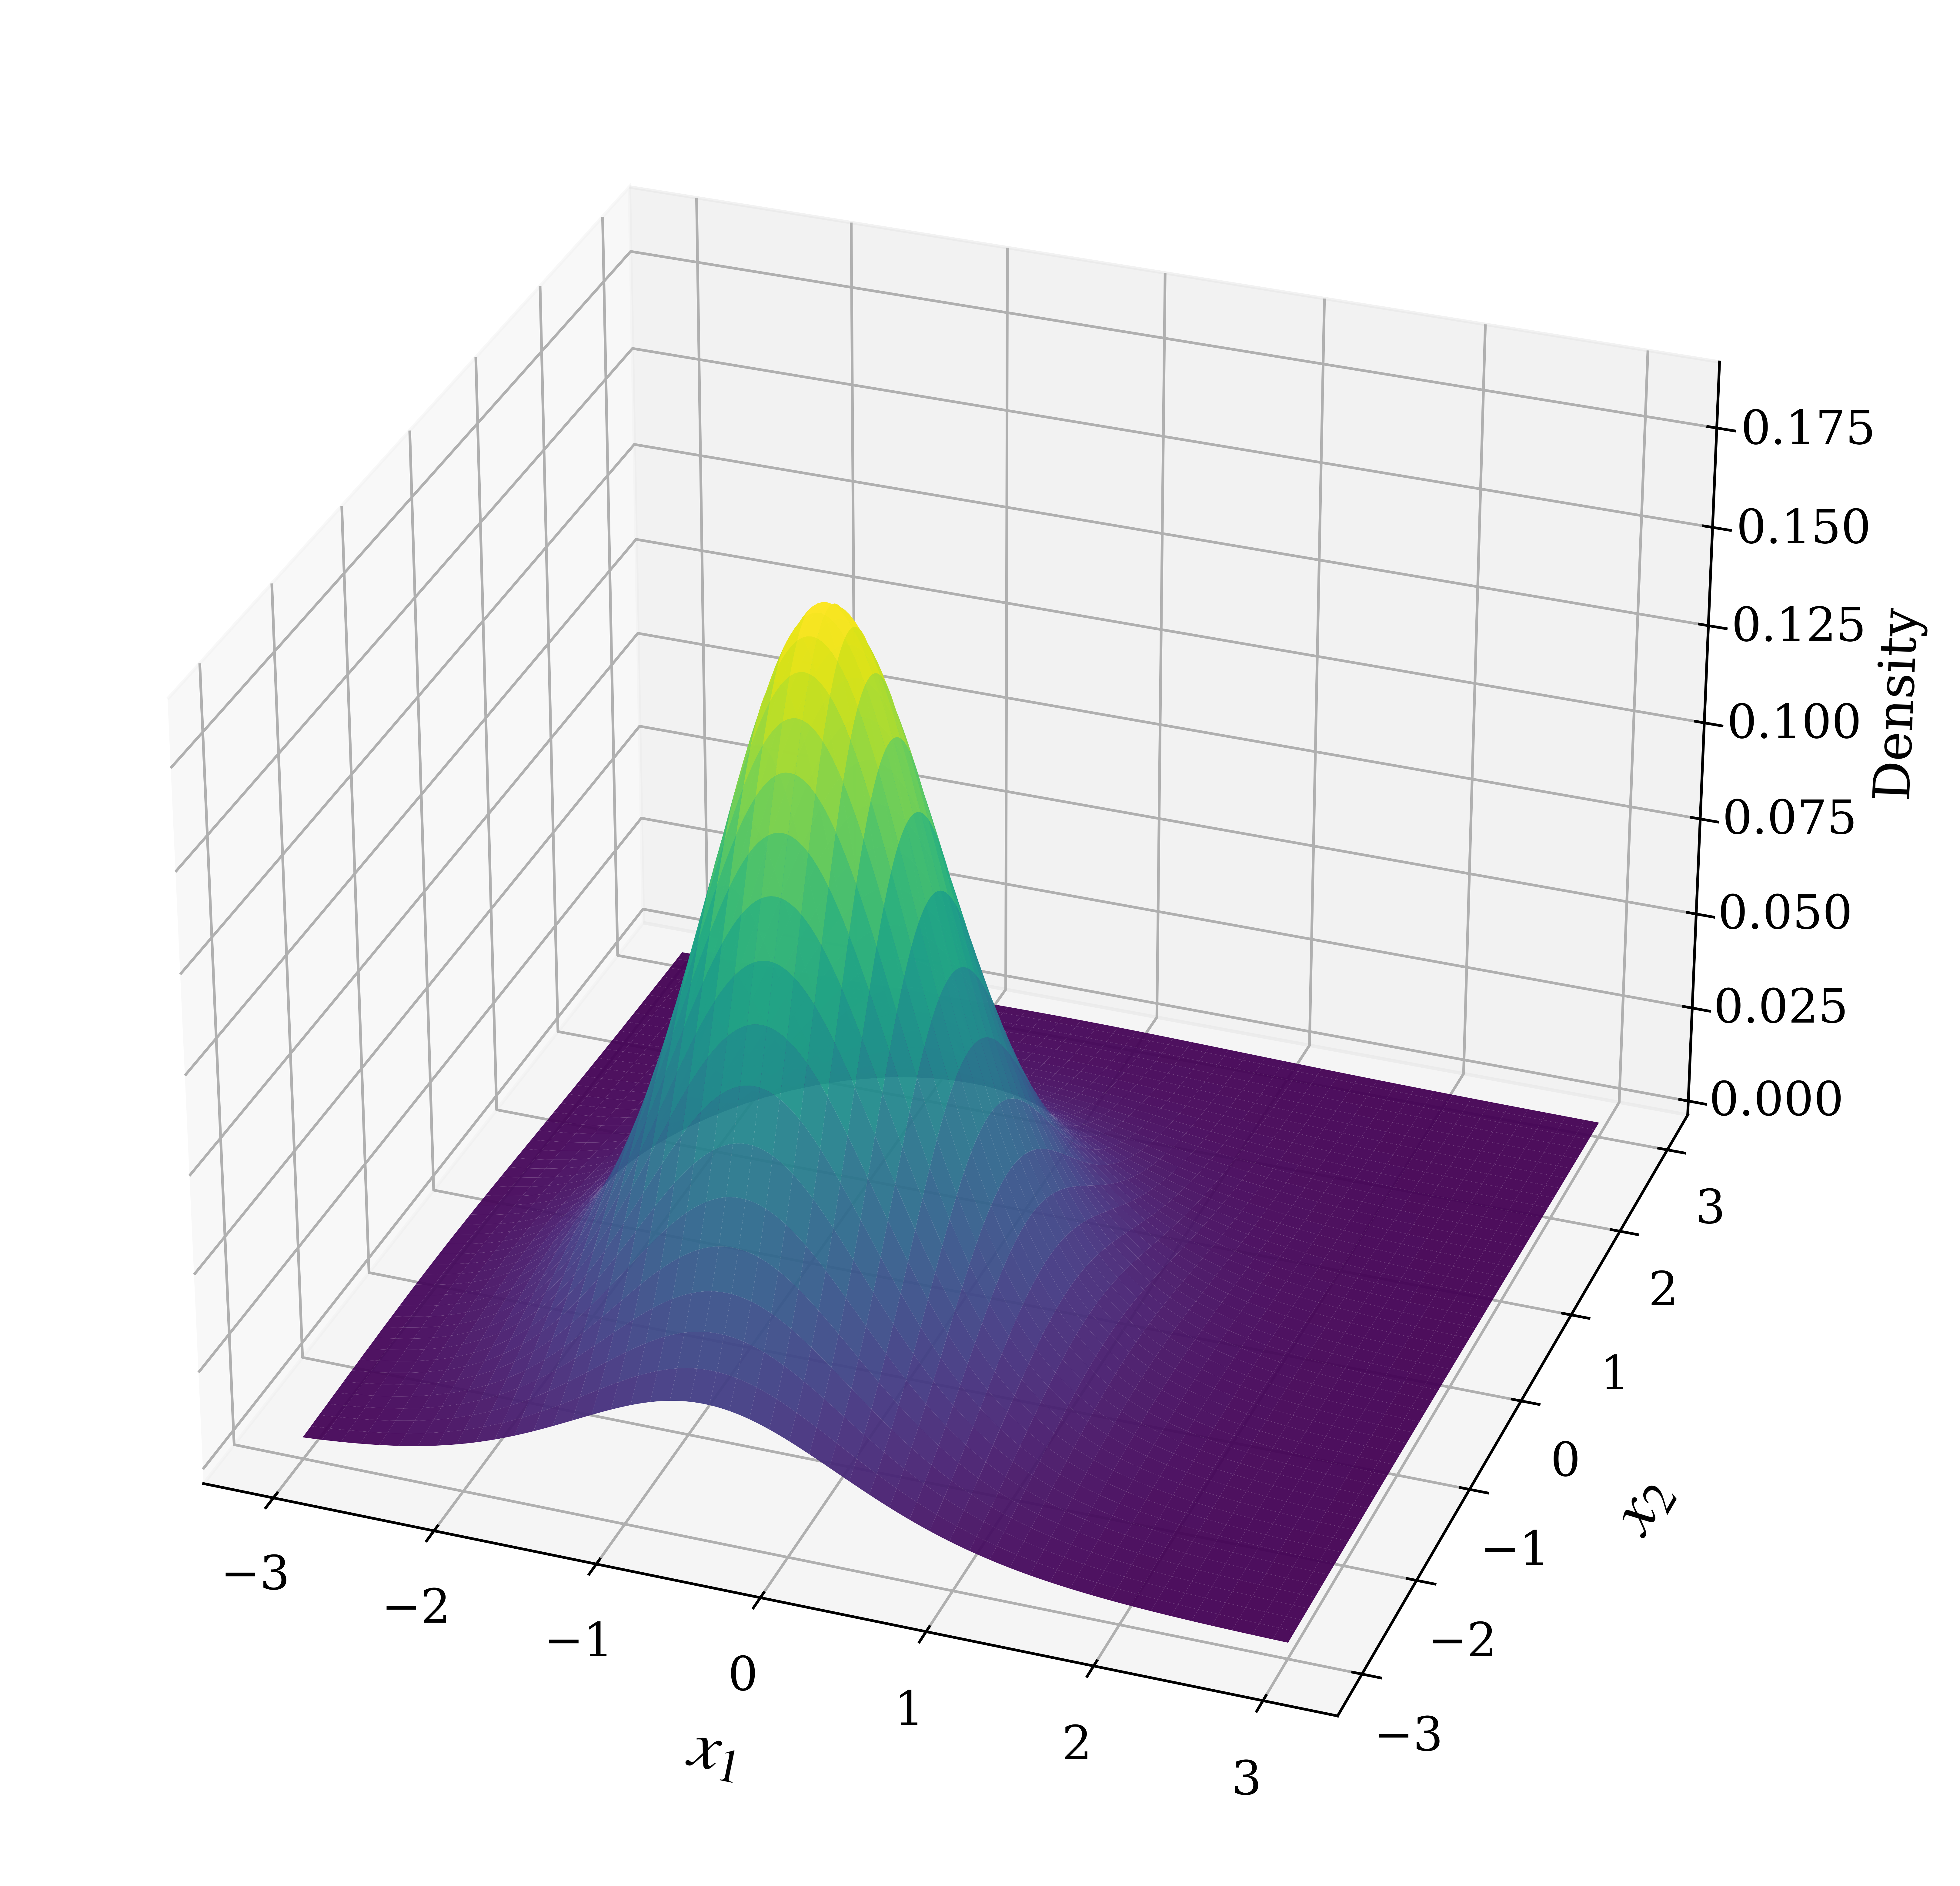
\includegraphics[width=0.5\linewidth]{figures/plot1.png}
    }
    \subfigure[$\;$ IGa-N$_d$ distribution;]
    {
        \centering
        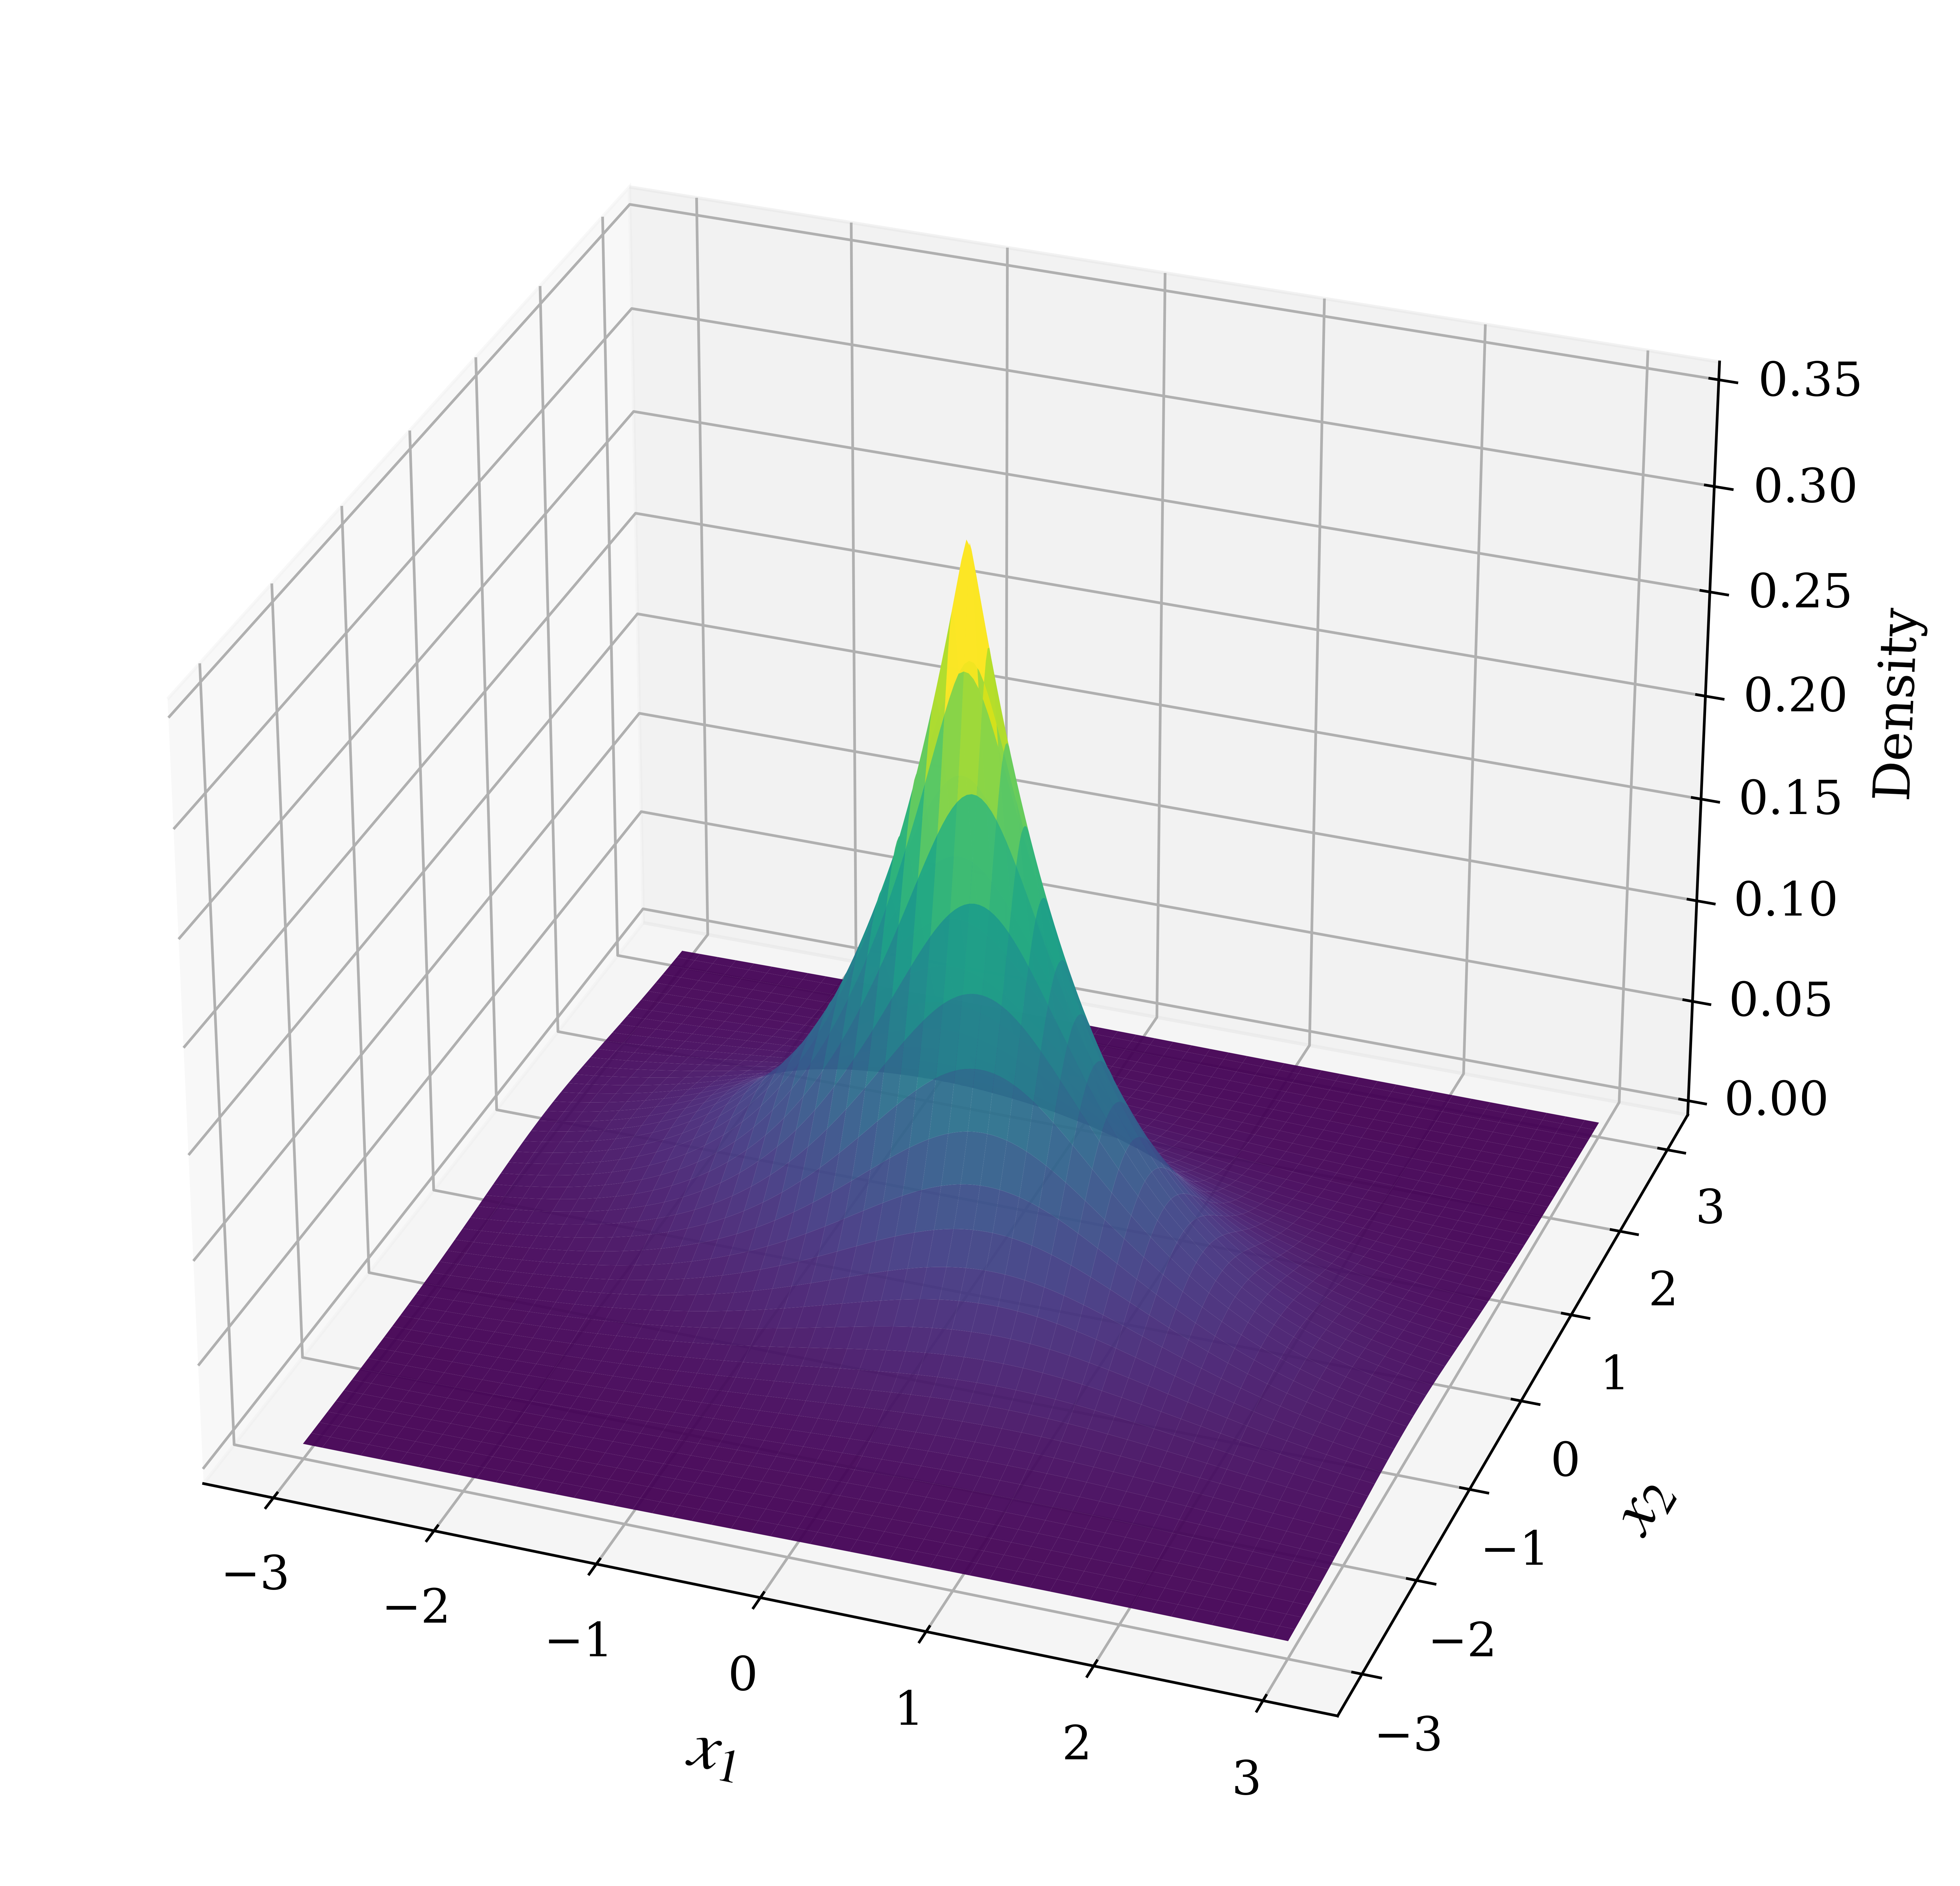
\includegraphics[width=0.5\linewidth]{figures/plot5.png}
    }
    \subfigure[$\;$ IGau-N$_d$ distribution.]
    {
        \centering
        
\includegraphics[width=0.5\linewidth]{figures/plot10.png}
    }
    \subfigure[$\;$ RIGau-N$_d$ distribution.]
    {
        \centering
        
\includegraphics[width=0.5\linewidth]{figures/plot15.png}
    }
    \caption{$\;$ Density of specific cases for Ge-N$_d$ family under various parameter combinations.}
    \label{zyf.four.fig1}
\end{figure}
\section{$\!\!\!\!\!\!\!$. Data--driven Non-parametric Mixtures and Oracle Property}       % Section 3

In \S\ref{zyf.four.sec:GeN}, we systematically construct the Ge-N$_d$ family by assuming mixture variable $\tau$ follows specific parametric distributions. However, in practical applications, the true underlying distribution of data generation process is typically unknown.  Pre-specifying a parametric form for $\tau$ may lead to model mis-specification, which can severely compromise the robustness of the statistical inference. To overcome this limitation, the following section introduces a data--driven approach. By employing non-parametric techniques to model the mixture variable, we propose a flexible and robust non-parametric mixture of multivariate normal distribution, which effectively eliminates the reliance on subjective parametric assumptions.

\subsection{Definition of NPM-N$_d$ distribution}\label{zyf.four.sec:NPMN.definition}       % Section 3.1

In this section, we do not specify the specific distribution of the mixture variable $\tau$ (i.e., no specific expression for $f_\tau(\tau|\bla)$), but adopt the right-endpoint histogram discretization method (see more details in Appendix \ref{zyf.four.sec:discretization}) to discretize \trv $\tau$ into
\begin{eqnarray}    \label{zyf.four.3.1}
    \Pr(\tau = \tau_j) = p_j, \quad j = 1, \dots, M \qor F_\tau(\tau|\ibp) = \sum_{j=1}^M p_j \cdot I(\tau \ge \tau_j),
\end{eqnarray}
where $\ibp = (p_1, \dots, p_M)^\top$ an unknown parameter vector of weights satisfying $\ibp \in \bbT_M$ with
$$
   \bbT_M \teq \left\{\ibp = (p_1, \dots, p_M)^{\T} \col 0 \le p_j \le 1, \; j = 1, \dots, M, \; \ibp^{\T}\1_M = 1 \right\},
$$
and $0 < \tau_1 < \cdots < \tau_M$ is a partition of interval $\bbR_+$. Then we provide the following definition.
\begin{definition}{\rm \textbf{(Non-parametric mixture of multivariate normal distribution).} Suppose that the mixture variable $\tau$ with the \textit{cumulative distribution function} (cdf) $F_\tau(\tau | \ibp)$ in (\ref{zyf.four.3.1}), where $\ibp = (p_1, \dots, p_M)^\top \in \bbT_M$ is an unknown weight parameter vector. If a $d$-dimensional continuous vector $\ibX = (X_1, \dots, X_d)^\top$ has the SR (\ref{zyf.four.2.1}) with $\ibZ = (Z_1, \dots, Z_d)^\top \sim N_d(\0, \bSi)$ with $\ibZ \inde \tau$. Then we say $\ibX$ follows the \textit{non-parametric mixture of multivariate normal} (NPM-N$_d$) distribution, denoted by $\ibX \sim \NPMN$ or $\mbox{NPM-N}_d(\bphi)$, where $\bphi = \{\bmu, \bSi, \ibp\}$ is the parameter vector with $\bmu \in \bbR^d$ is the location parameter and $\bSi = (\sigma_{ij})_{d \times d}$ is the scale parameter matrix. \hfill $\|$
}\end{definition}

For $\ibX \sim \mbox{NPM-N}_d(\bphi)$ , we easily obtain the joint pdf as
\begin{eqnarray}    \label{zyf.four.3.2}
    \mbox{NPM-N}_d(\ibx | \bphi) = \frac{\1_M^\top \ibh_*(\ibx | \bphi)}{(2\pi)^{d/2} |\bSi|^{1/2}},
\end{eqnarray}
where $\ibh_*(\ibx | \bphi) = (h_{1*}(\ibx | \bphi), \dots, h_{M*}(\ibx | \bphi))^\top$ with
\begin{eqnarray*}
    h_{j*}(\ibx | \bphi) \teq p_j \tau_j^{d / 2} \exp\left\{-\frac{\tau_j}{2} (\ibx - \bmu)^\top \bSi^{-1} (\ibx - \bmu)\right\}, \quad j = 1, \dots, M.
\end{eqnarray*}

\subsection{Mean regression model for $\NPMN$ distribution}\label{zyf.four.sec:NPMN.reg}        % Section 3.2

Assume that $\{\ibX_i\} \ind \mbox{NPM-N}_d(\bmu_i, \bSi, \ibp)$ and $\Y{obs} = \{\ibx_i, \ibzi\}_{i=1}^n$ denote the observed data, we consider the following mean regression model
\begin{eqnarray}    \label{zyf.four.3.3}
    E(\ibX_i) = \bmu_i = \bB^\top \ibzi, \quad i = 1, \dots, n,
\end{eqnarray}
where $\ibzi=(z_{i1}, \dots, z_{iq})^\top$ is a $q$-dimensional vector of covariates for the $i$-th subject, and the matrix of regression coefficients
$$
\bB = \left(
\begin{array}{cccc}
  \beta_{11} & \beta_{12} & \cdots & \beta_{1d} \\
  \beta_{21} & \beta_{22} & \cdots & \beta_{2d} \\
  \vdots     & \vdots     & \ddots & \vdots \\
  \beta_{q1} & \beta_{q2} & \cdots & \beta_{qd}
\end{array}
\right),
$$
with $q \times d + d(d + 1) / 2 + M\leq n$. Let $\bvp = \{\bB, \bSi, \ibp\}$ be the parameter vector. Based on (\ref{zyf.four.3.2}) and (\ref{zyf.four.3.3}), the log-likelihood function of $\bvp$ is
\begin{eqnarray}    \label{zyf.four.3.4}
    \mcL(\bvp | \Y{obs}) = -\frac{nd}{2}\log(2\pi) - \frac{n}{2} \log|\bSi| + \sum_{i=1}^n \log \left[\1_M^\top \ibh(\ibx_i | \bvp) \right],
\end{eqnarray}
where $\ibh(\ibx_i | \bvp) = (h_1(\ibx_i | \bvp), \dots, h_M(\ibx_i | \bvp))^\top$ for $i = 1, \dots, n$ with
\begin{eqnarray}    \label{zyf.four.3.5}
    h_j(\ibx_i | \bvp) = p_j \tau_j^{d / 2} \exp\left\{-\frac{\tau_j}{2} (\ibx_i - \bmu_i)^\top \bSi^{-1} (\ibx_i - \bmu_i)\right\}, \quad j = 1, \dots, M.
\end{eqnarray}
The aim of this subsection is to calculate the MLEs of $\bvp$ through an MM algorithm. To this end, we first note the discrete version of Jensen's inequality
$$
    \xi\left(\sum_{j=1}^M b_j z_j \right) \ge \sum_{j=1}^M b_j \xi(z_j),
$$
for any concave function $\xi(\cdot)$, where $\ibb=(b_1, \dots, b_M)^\top \in \bbT_{M}$. For a fixed $i$, by setting $\xi(\cdot) = \log(\cdot)$, we then have the following inequality
\begin{eqnarray}    \label{zyf.four.3.6}
   \log (\1_M^\top \ibh(\ibx_i | \bvp)) \ge \constant + \sum_{j=1}^M \gt{ij} \log h_j(\ibx_i | \bvp),
\end{eqnarray}
where the weights
\begin{eqnarray}    \label{zyf.four.3.7}
    \gt{ij} \teq \frac{h_j(\ibx_i | \bvpt)}{\sum_{j=1}^M h_j(\ibx_i | \bvpt)} = \frac{h_j(\ibx_i | \bvpt)}{\1_M^\top \ibh(\ibx_i | \bvpt)},
\end{eqnarray}
where $\bvpt$ represents the $t$-th approximation of the MLE $\hbvp$. By combining (\ref{zyf.four.3.4}) with (\ref{zyf.four.3.6}), we can construct a surrogate function as
$$
    Q(\bvp | \bvpt) = \constant - \frac{n}{2} \log|\bSi| + \sum_{i=1}^n \sum_{j=1}^M \gt{ij} \left[\log p_j - \frac{\tau_j}{2} (\ibx_i - \bmu_i)^\top \bSi^{-1} (\ibx_i - \bmu_i)\right],
$$
By maximizing $Q(\bvp | \bvpt)$ with respect to $\bvp$, we obtain the MM iterations as
\begin{eqnarray*}
    \bBtI &=& \left[\sum_{i=1}^n \left(\sum_{j=1}^M \gt{ij}\tau_j\right) \ibzi \ibzi^\top \right]^{-1} \left[\sum_{i=1}^n \left(\sum_{j=1}^M \gt{ij}\tau_j\right) \ibzi \ibx_i^\top \right] \\ [2mm]
    &=& (\bZ^\top \At{} \bZ)^{-1}(\bZ^\top \At{} \bX) \\ [2mm]
    \bSitI &=& \frac{1}{n} \sum_{i=1}^n \left(\sum_{j=1}^M \gt{ij}\tau_j\right) \left(\ibx_i - \bB^{(t+1)\top}\ibzi \right)\left(\ibx_i - \bB^{(t+1)\top}\ibzi \right)^\top \\ [2mm]
    &=& \frac{1}{n} \left(\bX - \bZ\bBtI\right)^\top \At{} \left(\bX - \bZ\bBtI \right) \\ [2mm]
    \ptI{j} &=& \frac{\sum_{i=1}^n \gt{ij}}{\sum_{j=1}^M \sum_{i=1}^n \gt{ij}} = \frac{\1_n^\top \ibgt{j}}{\1_n^\top \bG^{(t)} \1_M}, \quad j = 1, \dots, M,
\end{eqnarray*}
where the covariate matrix $\bZ = (\ibz_{(1)}, \dots, \ibz_{(n)})^\top$, $\bX = (\ibx_1, \dots, \ibx_n)^\top$, for $i = 1, \dots, n$, and $j = 1, \dots, M$, we define
\begin{eqnarray*}
    && \at{i} \teq \sum_{j=1}^M \gt{ij}\tau_j, \quad \At{} \teq \diag\{\at{1}, \dots, \at{n}\}, \\ [2mm]
    && \bG^{(t)} \teq (\gt{ij})_{n\times M} = (\ibgt{1}, \dots, \ibgt{M}) \qwi \ibgt{j} = \left(
    \begin{array}{c}
        \gt{1j}  \\
        \vdots \\
        \gt{nj}
    \end{array} \right)
\end{eqnarray*}
being the $j$-column of $\bG^{(t)}$, here $\gt{ij}$ is given by (\ref{zyf.four.3.7}). The MM iterations are repeated until
$$
   \bigg|\frac{\mcL(\bvptI|\Y{obs}) - \mcL(\bvpt|\Y{obs})} {\mcL(\bvpt|\Y{obs})}\bigg| \le \de_0.
$$
where $\de_0$ is a pre-specified small positive number.

\subsection{Adaptive hyper-parameter selection strategy}        % Section 3.3

When constructing the NPM-N$_d$ model, the selection of hyper-parameters (number of discrete intervals $M$, locations of support points $\{\tau_m\}_{m=1}^M$ with their initial weights $\ibp^{(0)}$) directly determines the flexibility and generalization capability of model fitting. To achieve an optimal balance between eliminating parametric mis-specification and avoiding over-fitting, we propose an adaptive hyper-parameter selection strategy that combines Gauss--Laguerre quadrature with cross-validation.

\subsubsection{Progressive screening mechanism for the number of discrete intervals}        % Section 3.3.1

The parameter $M$ controls the accuracy of the discrete approximation: an excessively small $M$ leads to insufficient fitting capacity, while an overly large $M$ triggers severe overfitting, manifested by artificially high likelihood values on the training set but a sharp decline in generalization ability. To address this, we design a progressive screening mechanism comprising three steps:

\begin{namelist}{01234567}
\item[\hspace{0.08cm} \tsf{Step 1:}]  Referring to the method of sieves, we do not allow $M$ to grow infinitely. Instead, we restrict it to a candidate set $M \in \{M_1, ..., M_T\}$ that grows moderately with the sample size $n$ (e.g., $M_t = O(n^\al)$, where $\al \in (0,1)$);

\item[\hspace{0.08cm} \tsf{Step 2:}]  We sequentially execute the MM algorithm over the candidate set and compute the relative likelihood gain brought by adjacent numbers of nodes, defined as 
$$
    \De(M_t) \teq \left|\frac{\mcL(M_{t+1}) - \mcL(M_t)}{\mcL(M_t)}\right|.
$$
When $M$ exceeds a certain threshold, the growth rate of the likelihood function significantly decelerates. Therefore, we select the smallest $M_t$ that satisfies $\Delta(M_t) < \ve$ (where $\ve$ is a pre-specified small positive tolerance), thereby eliminating redundant nodes with minimal marginal returns.

\item[\hspace{0.08cm} \tsf{Step 3:}]  To completely circumvent over-fitting, we introduce cross-validation based on the preliminary screening. The sample is partitioned into a training set and a testing set, and the \textit{mean absolute error} (MAE) is calculated on the testing set. Ultimately, the value of $M$ that minimizes $\mbox{MAE}_\text{test}$ is selected as the optimal hyper-parameter: 
$$
    M_{opt} = \arg\min_M \mbox{MAE}_\text{test}(M_t).
$$
\end{namelist}

\subsubsection{Heuristic determination of support points and initial weights}        % Section 3.3.2

Based on the Riemann--Stieltjes approximation, it is first necessary to reasonably allocate grid points within the domain of integration. Noting that the log-likelihood function of the NPM-N$_d$ involves an integral form with an exponential decay factor $e^{-\tau}$, i.e., 
\begin{eqnarray*}
    \ell_\tau(\bga | \Y{obs}) &=& \sum_{i=1}^n \log \int_0^\infty \tau^{d / 2} f_\tau(\tau|\bla) \exp\left(-\frac{Q_i\tau}{2}\right) \rd \tau \\ [2mm]
    &=& \sum_{i=1}^n \log \int_0^\infty \e^{-\tau} \tau^{d / 2} f_\tau(\tau|\bla) \exp\left[\left(1-\frac{Q_i}{2}\right)\tau\right] \rd \tau, 
\end{eqnarray*}
where quadratic form $Q_i = (\ibx_i - \bmu)^\top \bSi^{-1} (\ibx_i - \bmu)$, we introduce the Gauss--Laguerre quadrature (see Appendix \ref{zyf.four.sec:GLquadrature} for details) to determine the discrete grid.

For a given number of intervals $M$, we directly extract the $M$ nodes of the Gauss--Laguerre polynomial, denoted as $\{\tau_m\}_{m=1}^M$, to serve as the fixed discrete support points for the mixture variable $\tau$, and utilize their corresponding quadrature weights $\{p_m\}_{m=1}^M$ as the initial values $\ibp^{(0)}$ for the discrete probabilities. This selection strategy has the advantages of covering the core area of the integral and improving the computational stability.

\subsection{Likelihood approximation via Riemann--Stieltjes integral}\label{zyf.four.sec:Likelihoodapproximation}     % Section 3.4

Suppose that $\{\ibX_i\}_{i=1}^n \iid \GeN$ with a specific mixture variable $\tau$ and mixture density $f_\tau(\tau|\bla)$ satisfying there exists a constant $S$ large enough such that the probability $\Pr(\tau \in [0, S] > 1 - \ve)$ holds for any $\ve > 0$. Denote $\Y{obs} = \{\ibx_i\}_{i=1}^n$ be the observed data, we easily obtain the log-likelihood function of $\bga = \{\bmu, \bSi, \bla\}$ as
\begin{eqnarray} \label{zyf.four.3.8}
    \ell(\bga | \Y{obs}) \sr{(\ref{zyf.four.2.10})} -\frac{nd}{2}\log(2\pi) - \frac{n}{2}\log|\bSi| + \ell_\tau(\bga | \Y{obs}),
\end{eqnarray}
where
\begin{eqnarray*}
    \ell_\tau(\bga | \Y{obs}) = \sum_{i=1}^n \log \int_0^\infty \tau^{d / 2} f_\tau(\tau|\bla) \exp\left[-\frac{\tau}{2} \left(\ibx_i - \bB^\top\ibzi \right)^\top \bSi^{-1} \left(\ibx_i - \bB^\top\ibzi \right)\right] \rd \tau.
\end{eqnarray*}
We further assume that there exists a partition on the interval $[0, S]$, denoted by $M$ disjoint sub-intervals as $\bbS_j = (\tau_{j - 1}, \tau_j]$ with $0 = \tau_0 < \tau_1 < \cdots < \tau_M = S$, the partition mesh size satisfies $\|\Pi\| = \max_{1 \le j \le M} (\tau_j - \tau_{j - 1}) \to 0$ as $M \to \infty$. Then by employing the Riemann--Stieltjes approximation (\ref{zyf.four.A.3}), we approximate $\ell_\tau(\bga | \Y{obs})$ as
\begin{eqnarray*}
    \ell_\tau(\bga | \Y{obs}) &\ap& \sum_{i=1}^n \log \sum_{j=1}^M \int_{\bbS_j} \tau^{d / 2} f_\tau(\tau|\bla) \exp\left[-\frac{\tau}{2} \left(\ibx_i - \bB^\top\ibzi \right)^\top \bSi^{-1} \left(\ibx_i - \bB^\top\ibzi \right)\right] \rd \tau \\ [2mm]
    &\ap& \sum_{i=1}^n \log \sum_{j=1}^M p_j \tau_j^{d / 2} \exp\left[-\frac{\tau_j}{2} \left(\ibx_i - \bB^\top\ibzi \right)^\top \bSi^{-1} \left(\ibx_i - \bB^\top\ibzi \right)\right],
\end{eqnarray*}
where $p_j = \int_{\bbS_j} f(\tau|\bla) \rd \tau$. Review the definition of $h_j(\ibx | \bvp)$ in (\ref{zyf.four.3.5}), we found that the log-likelihood function of $\bga$ can be approximated as
\begin{eqnarray*}
    \ell(\bga | \Y{obs}) &=& -\frac{nd}{2}\log(2\pi) - \frac{n}{2}\log|\bSi| + \ell_\tau(\bga | \Y{obs}) \\ [2mm]
    &\ap& -\frac{nd}{2}\log(2\pi) - \frac{n}{2}\log|\bSi| + \sum_{i=1}^n \log \left[\1_M^\top \ibh(\ibx_i | \bvp) \right] \\ [2mm]
    &\sr{(\ref{zyf.four.3.4})}& \mcL(\bvp | \Y{obs}),
\end{eqnarray*}
which is actually the log-likelihood function of NPM-N$_d$ in \S\ref{zyf.four.sec:NPMN.reg}. Therefore, the proposed NPM-N$_d$ distribution is equivalent to the likelihood approximation of the original parameterized Ge-N$_d$ distribution via Riemann--Stieltjes integral.
\section{$\!\!\!\!\!\!\!$. Simulation Studies}    % Section 4

\subsection{Accuracy of point estimators}       % Section 4.1

To investigate the accuracy of MLE and \textit{moment estimator} (ME) for $\GeN$ distributions and assess the performance of these two methods, we employ the \textit{mean square error} (\tsf{MSE}) and log-likelihood value (\tsf{Loglikelihood}) to evaluate the goodness of fit.

In our simulations, we consider different sample sizes $n = 300(300)900$ and $R = 10$,000 sampling replications. We conduct the numerical experiments with following four cases:
\begin{namelist}{0123456789}
\item[\hspace*{-0.05cm} Case (A$_1$):] Independently generating $\{\ibX_i^{(r)}\}_{i=1}^n \iid \mbox{Ga-N}_2(\bmu, \bSi, \la)$ with the true values being set as $\bmu = (-1, 2)^\top$, $\bSi = (1, 0.5; 0.5, 2)$ and $\la = 2.5$;

\item[\hspace*{-0.05cm} Case (A$_2$):] Independently generating $\{\ibX_i^{(r)}\}_{i=1}^n \ind \mbox{IGa-N}_2(\bmu_i, \bSi, \la)$ with true values being set as $\bB = (2, 0; -1, 0.5; 0, -3)$, $\bSi = (1, 0.5; 0.5, 2)$ and $\la = 1.5$;

\item[\hspace*{-0.05cm} Case (A$_3$):] Independently generating $\{\ibX_i^{(r)}\}_{i=1}^n \iid \mbox{IGau-N}_2(\bmu, \bSi, \la)$ with the true values being set as $\bmu = (0.5, -1)^\top$, $\bSi = (2, -0.5; -0.5, 1)$ and $\la = 2$;

\item[\hspace*{-0.05cm} Case (A$_4$):] Independently generating $\{\ibX_i^{(r)}\}_{i=1}^n \ind \mbox{RIGau-N}_2(\bmu_i, \bSi, \la)$ with true values being set as $\bB = (0, 2; 1, -1; -3, 0)$, $\bSi = (0.5, 0.75; 0.75, 2.5)$ and $\la = 0.5$.
\end{namelist}

Given a combination of $\{n, r, \bmu, \bSi, \la\}$ for Case (A$_1$), let $\Y{obs}^{(r)} = \{\ibx_i^{(r)}\}_{i=1}^n$ denote the $r$-th observations with $r = 1, \dots, R$, where $\ibx_i^{(r)}$ is a realization of $\ibX_i^{(r)}$. We can compute the MLEs of parameters via N-EM algorithm, denoted by $\{\hbmu^{(r)}, \hbSi^{(r)}, \hla^{(r)}\}$ and MEs, denoted by $\{\hbmu_M^{(r)}, \hbSi_M^{(r)}, \hla_M^{(r)}\}$. Next, we calculate the \textit{average MLE} (\tsf{A-MLE}) and the \textit{average ME} (\tsf{A-ME}) with the corresponding \tsf{MSE} for each parameter based on the $R$ repetitions. The above results of Case (A$_1$) are summarized in Table \ref{zyf.four.tab1}.

\newpage
\vkU
\baselineskip 0.10in
\begin{Table} \label{zyf.four.tab1} {\rm  \ \  \hspace*{-0.5cm}{\bf .}
Comparisons of \tsf{A-MLE}s, \tsf{A-ME}s with corresponding \tsf{MSE} for Case (A$_1$) under various sample sizes
\vspace{-0.3cm}
\begin{center}
\renewcommand{\arraystretch}{1.2} \tabcolsep 0.07in \doublerulesep 0.2pt
\begin{tabular}{clcrrrrrr}  \hline\hline
    \MR{2}{*}{Size} & \MR{2}{*}{Method} & \MR{2}{*}{\tsf{Loglikelihood}} & \MC{6}{c}{Parameter} \\ \cline{4-9}
    \MR{2}{*}{}     & \MR{2}{*}{}       & \MR{2}{*}{}                    & \MC{1}{c}{$\mu_1$}   & \MC{1}{c}{$\mu_2$} & \MC{1}{c}{$\sigma_{11}$} & \MC{1}{c}{$\sigma_{11}$} & \MC{1}{c}{$\sigma_{11}$} & \MC{1}{c}{$\la$} \\ \hline
    \MR{4}{*}{300}  & \MR{2}{*}{MLE}    & \MR{2}{*}{$-$899.401}          & $-$0.9999            & 1.9996             & 1.0056                   & 0.5020                   & 2.0087                   & 2.6975           \\
    \MR{4}{*}{}     & \MR{2}{*}{}       & \MR{2}{*}{}                    & (0.0026)             & (0.0053)           & (0.0179)                 & (0.0123)                 & (0.0710)                 & (0.5420)         \\ 
    \MR{4}{*}{}     & \MR{2}{*}{ME}     & \MR{2}{*}{$-$901.712}          & $-$1.000             & 1.9997             & 1.0019                   & 0.4990                   & 1.9999                   & 3.4868           \\
    \MR{4}{*}{}     & \MR{2}{*}{}       & \MR{2}{*}{}                    & (3.5e-5)             & (0.0001)           & (0.0253)                 & (0.0222)                 & (0.0956)                 & (2.4406)         \\ \hdashline
    \MR{4}{*}{600}  & \MR{2}{*}{MLE}    & \MR{2}{*}{$-$1801.611}         & $-$0.9996            & 2.0004             & 1.0030                   & 0.5013                   & 2.0050                   & 2.5829           \\
    \MR{4}{*}{}     & \MR{2}{*}{}       & \MR{2}{*}{}                    & (0.0013)             & (0.0026)           & (0.0084)                 & (0.0059)                 & (0.0333)                 & (0.1727)         \\ 
    \MR{4}{*}{}     & \MR{2}{*}{ME}     & \MR{2}{*}{$-$1804.570}         & $-$0.9996            & 2.0000             & 1.0021                   & 0.5008                   & 2.0029                   & 3.1404           \\
    \MR{4}{*}{}     & \MR{2}{*}{}       & \MR{2}{*}{}                    & (9.0e-6)             & (3.2e-5)           & (0.0158)                 & (0.0142)                 & (0.0561)                 & (0.7904)         \\ \hdashline
    \MR{4}{*}{900}  & \MR{2}{*}{MLE}    & \MR{2}{*}{$-$2702.718}         & $-$0.9997            & 2.0003             & 1.0005                   & 0.5005                   & 2.0003                   & 2.5579           \\
    \MR{4}{*}{}     & \MR{2}{*}{}       & \MR{2}{*}{}                    & (9.0e-4)             & (0.0018)           & (0.0055)                 & (0.0039)                 & (0.0222)                 & (0.1064)         \\ 
    \MR{4}{*}{}     & \MR{2}{*}{ME}     & \MR{2}{*}{$-$2706.116}         & $-$0.9998            & 2.0004             & 1.0013                   & 0.5004                   & 2.0011                   & 3.0205           \\
    \MR{4}{*}{}     & \MR{2}{*}{}       & \MR{2}{*}{}                    & (4.0e-6)             & (1.5e-5)           & (0.0097)                 & (0.0093)                 & (0.1089)                 & (0.5124)         \\ \hline\hline
\end{tabular}
\end{center} }
\end{Table}
\vspace{-0.3cm}
\noi  {\small  The MSEs corresponding to MLE and ME are shown in parentheses. \\
               The convergence accuracy of MLE is $10^{-8}$.}
\baselineskip 0.30in

\vkL
For the Case (A$_2$) and (A$_4$) with covariate, we independently generate $\ibzi^{(r)} = (1, z_{1i}^{(r)}, z_{2i}^{(r)})^\top$ with
$$
    z_{1i}^{(r)} \iid N(0, 1) \qand z_{12}^{(r)} \iid \Poisson(2), \qfor i = 1, \dots, n.
$$
The \tsf{Loglikelihood}, \tsf{A-MLE} and corresponding \tsf{MSE} for Case (A$_4$) are presented in Table \ref{zyf.four.tab2}. We found that with the increase of sample size $n$, the MLEs and MEs of parameters becomes more and more accurate and stable. Specifically, \tsf{A-MLE} and \tsf{A-ME} is getting closer to the set true value, and \tsf{MSE} is getting smaller. Similar conclusions were reached in Case (A$_2$) and (A$_3$), we summarized the results into tables and displayed them in the \hyperref[zyf.four.sec:SM]{Supplementary Materials} for reading.

\newpage
\vkU
\baselineskip 0.10in
\begin{Table} \label{zyf.four.tab2} {\rm  \ \  \hspace*{-0.5cm}{\bf .}
Comparisons of \tsf{Loglikelihood}, \tsf{A-MLE}s with corresponding \tsf{MSE} for Case (A$_4$) under various sample sizes
\vspace{-0.3cm}
\begin{center}
\renewcommand{\arraystretch}{1.2} \tabcolsep 0.135in \doublerulesep 0.2pt
\begin{tabular}{crcrr}  \hline\hline
    Size           & \tsf{Loglikelihood}  & Parameter & \MC{1}{c}{\tsf{A-MLE}}                                                                                & \MC{1}{c}{\tsf{MSE}}                                                                                 \\ \hline
    \MR{3}{*}{300} & \MR{3}{*}{$-$712.5871} & $\bB$     & $\left(\begin{array}{rr} -0.0007 & 1.9977 \\ 0.9996 & -1.0013 \\ -2.9998 & 0.0008 \end{array}\right)$ & $\left(\begin{array}{rr} 0.0027 & 0.0136 \\ 0.0009 & 0.0045 \\ 0.0005 & 0.0022 \end{array}\right)$ \\
    \MR{3}{*}{}    & \MR{3}{*}{}            & $\bSi$    & $\left(\begin{array}{rr} 0.4996 & 0.7494 \\ 0.7494 & 2.4995 \end{array}\right)$                       & $\left(\begin{array}{rr} 0.0051 & 0.0147 \\ 0.0147 & 0.1277 \end{array}\right)$                    \\
    \MR{3}{*}{}    & \MR{3}{*}{}            & $\la$     & 0.5186                                                                                                & 0.0189                                                                                             \\ \hdashline
    \MR{3}{*}{600} & \MR{3}{*}{$-$1430.651} & $\bB$     & $\left(\begin{array}{rr} 0.0003 & 2.0009 \\ 0.9998 & -1.0003 \\ -3.0001 & -0.0002 \end{array}\right)$ & $\left(\begin{array}{rr} 0.0013 & 0.0004 \\ 0.0067 & 0.0022 \\ 0.0002 & 0.0011 \end{array}\right)$ \\
    \MR{3}{*}{}    & \MR{3}{*}{}            & $\bSi$    & $\left(\begin{array}{rr} 0.5005 & 0.7511 \\ 0.7511 & 2.5046 \end{array}\right)$                       & $\left(\begin{array}{rr} 0.0026 & 0.0075 \\ 0.0075 & 0.0651 \end{array}\right)$                    \\
    \MR{3}{*}{}    & \MR{3}{*}{}            & $\la$     & 0.5080                                                                                                & 0.0084                                                                                             \\ \hdashline
    \MR{3}{*}{900} & \MR{3}{*}{$-$2147.333} & $\bB$     & $\left(\begin{array}{rr} -0.0003 & 1.9992 \\ 0.9999 & -1.0003 \\ -2.9998 & 0.0004 \end{array}\right)$ & $\left(\begin{array}{rr} 0.0009 & 0.0043 \\ 0.0003 & 0.0015 \\ 0.0001 & 0.0007 \end{array}\right)$ \\
    \MR{3}{*}{}    & \MR{3}{*}{}            & $\bSi$    & $\left(\begin{array}{rr} 0.5002 & 0.7507 \\ 0.7507 & 2.4997 \end{array}\right)$                       & $\left(\begin{array}{rr} 0.0017 & 0.0049 \\ 0.0049 & 0.0420 \end{array}\right)$                    \\
    \MR{3}{*}{}    & \MR{3}{*}{}            & $\la$     & 0.5057                                                                                                & 0.0054                                                                                             \\ \hline\hline
\end{tabular}
\end{center} }
\end{Table}
\vspace{-0.3cm}
\noi  {\small   The convergence accuracy of MLE is $10^{-8}$.}
\baselineskip 0.30in

\subsection{Bayesian estimation and credit interval}        % Section 4.2

This section, we conducts simulation studies to evaluate the finite--sample performance of the proposed ECM and DA algorithms in \S\ref{zyf.four.sec:Bayesian}, specifically focusing on the accuracy of posterior modes, posterior means, and the reliability of Bayesian credible intervals. We consider the size of $n = 500$ with $R = 1000$ independent replications for each scenario. To comprehensively evaluate the algorithms under diverse data structures, we examine four distinct distributions characterized by different parameter configurations:
\begin{namelist}{0123456789}
\item[\hspace*{-0.05cm} Case (B$_1$):] Independently generating $\{\ibX_i^{(r)}\}_{i=1}^n \iid \mbox{Ga-N}_2(\bmu, \bSi, \la)$ with true values $\bmu = (-1, 2)^\top$, $\bSi = (1, -0.5; -0.5, 2)$ and $\la = 2.5$ and conjugate prior;

\item[\hspace*{-0.05cm} Case (B$_2$):] Independently generating $\{\ibX_i^{(r)}\}_{i=1}^n \iid \mbox{IGa-N}_2(\bmu, \bSi, \la)$ with true values $\bmu = (0, -1)^\top$, $\bSi = (1, 0.5; 0.5, 1)$ and $\la = 1.5$ and conjugate prior;

\item[\hspace*{-0.05cm} Case (B$_3$):] Independently generating $\{\ibX_i^{(r)}\}_{i=1}^n \iid \mbox{IGau-N}_2(\bmu, \bSi, \la)$ with true values $\bmu = (1, 1)^\top$, $\bSi = (1, 0; 0, 1)$, $\la = 2$ and non-information prior;

\item[\hspace*{-0.05cm} Case (B$_4$):] Independently generating $\{\ibX_i^{(r)}\}_{i=1}^n \iid \mbox{RIGau-N}_2(\bmu, \bSi, \la)$ with true values $\bmu = (-1, 0)^\top$, $\bSi = (2, 0.75; 0.75, 1)$ and $\la = 0.5$ and non-information prior.
\end{namelist}
Given a combination of $\{n, r, \bmu, \bSi, \la\}$ for Case (B$_1$), we generate the observed data $\Y{obs}^{(r)} = \{\ibx_i^{(r)}\}_{i=1}^n$ and compute the MLE $\hla^{(r)}$ via N-EM algorithm. By fixing $\hla^{(r)}$ in Ga-N$_2$ distributions, we calculate the posterior mode $\{\tilde{\bmu}^{(r)}, \tilde{\bSi}^{(r)}\}$, generate the posterior sample and obtain the posterior mean $\{\bar{\bmu}^{(r)}, \bar{\bSi}^{(r)}\}$ with their 95\% Bayesian CIs. The conjugate prior is set as
$$
    (\bmu, \bSi) \sim \NIW_d(\bmu_0, \ka_0, \bLa_0, \nu_0),
$$
where $\bmu_0 = \hbmu_M^{(r)}$, $\ka_0 = 0.1$, $\bLa_0 = \hbSi_M^{(r)}$ and $\nu_0 = 4$. To characterize the accuracy of Bayesian estimation and the reliability of CIs, we adopt \tsf{MSE} and interval \textit{coverage rate} (\tsf{CR}) as evaluation criterion.

\vkU
\baselineskip 0.10in
\begin{Table} \label{zyf.four.tab3} {\rm  \ \  \hspace*{-0.5cm}{\bf .}
Bayesian estimations and CIs of parameters $\{\bmu, \bSi\}$ with \tsf{MSE} and \tsf{CR} for Case (B$_2$) and Case (B$_3$)
\vspace{-0.3cm}
\begin{center}
\renewcommand{\arraystretch}{1.2} \tabcolsep 0.08in \doublerulesep 0.2pt
\begin{tabular}{ccrrrrrr}  \hline\hline
    Case               & Parameter     & \makecell[c]{Posterior \\ Mode} & \makecell[c]{\tsf{MSE} for \\ Mode} & \makecell[c]{Posterior \\ Mean} & \makecell[c]{\tsf{MSE} for \\ Mean} & \MC{1}{c}{Bayesian CI}          & \MC{1}{c}{\tsf{CR}} \\ \hline
    \MR{5}{*}{(B$_2$)} & $\mu_1$       & $-$0.0009                       & 0.0015                              & $-$0.0009                       & 0.0015                              & $[-0.0727, 0.0707]$             & 0.9347              \\
    \MR{5}{*}{}        & $\mu_2$       & $-$0.9997                       & 0.0015                              & $-$0.9998                       & 0.0015                              & $[-1.0717, -0.9279]$            & 0.9347              \\
    \MR{5}{*}{}        & $\sigma_{11}$ & 0.9639                          & 0.0080                              & 0.9890                          & 0.0078                              & $[0.8385, 1.1523]$              & 0.9328              \\
    \MR{5}{*}{}        & $\sigma_{12}$ & 0.4806                          & 0.0039                              & 0.4897                          & 0.0039                              & $[0.3815, 0.6149]$              & 0.9441              \\
    \MR{5}{*}{}        & $\sigma_{22}$ & 0.9693                          & 0.0076                              & 1.0005                          & 0.0072                              & $[0.8433, 1.1588]$              & 0.9375              \\ \hdashline
    \MR{5}{*}{(B$_3$)} & $\mu_1$       & 0.9997                          & 0.0014                              & 0.9998                          & 0.0014                              & $[0.9243, 1.0752]$              & 0.9583              \\
    \MR{5}{*}{}        & $\mu_2$       & 1.0012                          & 0.0015                              & 1.0011                          & 0.0015                              & $[0.9258, 1.0764]$              & 0.9527              \\
    \MR{5}{*}{}        & $\sigma_{11}$ & 1.0032                          & 0.0077                              & 1.0105                          & 0.0092                              & $[0.8623, 1.1852]$              & 0.9233              \\
    \MR{5}{*}{}        & $\sigma_{12}$ & 0.0006                          & 0.0027                              & $-$0.0041                       & 0.0024                              & $[-0.1022, 0.1033]$             & 0.9498              \\
    \MR{5}{*}{}        & $\sigma_{22}$ & 0.9995                          & 0.0079                              & 0.9999                          & 0.0085                              & $[0.8591, 1.1809]$              & 0.9167              \\ \hline\hline
\end{tabular}
\end{center} }
\end{Table}
\vspace{-0.3cm}
\noi  {\small   The convergence accuracy of MLE is $10^{-8}$.}
\baselineskip 0.30in

The results for Case (B$_2$) and (B$_3$) are presented in Table \ref{zyf.four.tab3} above. The similar conclusions obtained from (B$_1$) and (B$_4$) are supplemented in the \hyperref[zyf.four.sec:SM]{Supplementary Materials}. We found that the posterior mode and mean is closed to the set true value, and \textsf{MSE} is small. For interval estimation, the \textsf{CR} is slightly lower than 95\% due to the small sample size. Overall, the Bayesian estimations and CIs are very accurate and reliable.


\subsection{Model comparison and robustness of NPM-N$_d$ distribution}       % Section 4.3

To assess the performance of the goodness-of-fit tests among the four specific distributions (i.e., Ga-N$_d$, IGa-N$_d$, IGau-N$_d$ and RIGau-N$_d$) of the Ge-N$_d$ family, we adopt \textit{Kullback--Leibler} (KL) divergence, \textit{integrated squared error} (ISE) and MSE as the evaluation criteria, which can be computed as
\begin{eqnarray*}
    \KL\left( f_{\rm true} \| \hf{\rm model} \right) &=& \int_{\bbR^d} f_{\rm true}(\ibx) \log \left[\frac{f_{\rm true}(\ibx)}{\hf{\rm model}(\ibx)}\right] \rd \ibx \ap \frac{1}{N} \sum_{i=1}^N \log \left[\frac{f_{\rm true}(\ibx_i)}{\hf{\rm model}(\ibx_i)}\right], \\ [2mm]
    \ISE\left(\hf{\rm model}\right) &=& \int_{\bbR^d} \left[ f_{\rm true}(\ibx) - \hf{\rm model}(\ibx) \right]^2 \rd \ibx \ap \frac{1}{N} \sum_{i=1}^N \frac{ \left[ f_{\rm true}(\ibx_i) - \hf{\rm model}(\ibx_i) \right]^2}{f_{\rm true}(\ibx_i)}, \\ [2mm]
    \MSE_{\rm pred}\left(\hf{\rm model}\right) &=& \frac{1}{N} \sum_{i=1}^N \|\ibx_{{\rm test}, i} - \hbmu_i\|_2^2,
\end{eqnarray*}
where $f_{\rm true}$ is the true density, $\hf{\rm model}$ is the fitting density of alternative model and $\{\ibx_{{\rm test}, i}\}_{i=1}^N$ are the samples in test set with size $N$.

In our numerical studies, the sample size, the number of sampling replications are respectively set to be $n = 500$ and $R = 10$,000. We set the parameters $\bB = (1, 0; -2.5, 1.5; 0, -2)$, $\bSi = (1, 0.5; 0.5, 2)$ and $\la$ in each of the four specific distributions (denoted by $\Two{\la}{Ga}$, $\Two{\la}{IGa}$, $\Two{\la}{IGau}$, $\Two{\la}{RIGau}$, respectively) can be determined by the common marginal kurtosis $\Kurt(X_j) = 2$. For a given $\{n, r, \bB, \bSi, \Kurt(X_j)\}$ with $r = 1, \dots, R$, firstly, we independently generate the covariate $\ibzi^{(r)} = (1, z_{1i}^{(r)}, z_{2i}^{(r)})^\top$ with
$$
    z_{1i}^{(r)} \iid N(0, 1) \qand z_{12}^{(r)} \iid \Poisson(2), \qfor i = 1, \dots, n,
$$
and the samples $\{\ibX_i^{(r)} = \ibx_i^{(r)}\}_{i=1}^n$ from the mixed distribution:
\begin{eqnarray*}
    && p_1 \cdot \mbox{Ga-N}_d(\bmu_i^{(r)}, \bSi, \Two{\la}{Ga}) + p_2 \cdot \mbox{IGa-N}_d(\bmu_i^{(r)}, \bSi, \Two{\la}{IGa}) + p_3 \cdot \mbox{IGau-N}_d(\bmu_i^{(r)}, \bSi, \Two{\la}{IGau}) \\ [2mm]
    && +\; p_4 \cdot \mbox{RIGau-N}_d(\bmu_i^{(r)}, \bSi, \Two{\la}{RIGau}),
\end{eqnarray*}
where the location parameter $\bmu_i^{(r)} = \bB^\top \ibzi^{(r)}$. The weights $p_s \ge 0$ for $s = 1, \dots, 4$ with $\sum_{s=1}^4 p_s = 1$. We consider the following situations for selecting $\ibp = (p_1, \dots, p_4)^\top$:
\begin{namelist}{0123456789}
\item[\hspace*{-0.05cm} Case (C$_1$):] Single--component distribution: $p_s = 1$ for $s = 1, \dots, 4$ and $p_{s'} = 0$ with $s'\ne s$, indicating that the sample is generated from each of four specific distributions;

\item[\hspace*{-0.05cm} Case (C$_2$):] Dominant two--component mixture distribution: One $p_s = 0.8$, the second $p_{s'} = 0.2$ for $s \ne s'$, and all others are zeros;

\item[\hspace*{-0.05cm} Case (C$_3$):] Uniform five--component mixed distribution: $\ibp=1/4\times\1_4$;

\item[\hspace*{-0.05cm} Case (C$_4$):] Dominant one--component mixed distribution: One specific case of Ge-N$_2$ distribution has a larger weight $p_s = 0.7$ and all others have smaller weights $p_{s'} = 0.1$.
\end{namelist}

Based on the generated sample $\{\ibx_i^{(k)} \}_{i=1}^n$, we randomly divided them into training set and test set at a ratio of $4:1$. Then we compute the MLEs $\{\hbB^{(r)}, \hbSi^{(r)}, \hla^{(r)}\}$ for the four specific distributions of the Ge-N$_2$ family via the N-EM algorithm on training set, calculate four KL divergence values $\{\tsf{KL}_1^{(r)}, \dots, \tsf{KL}_4^{(r)}\}$, ISE values $\{\tsf{ISE}_1^{(r)}, \dots, \tsf{ISE}_4^{(r)}\}$ and MSE values $\{\tsf{MSE}_1^{(r)}, \dots, \tsf{MSE}_4^{(r)}\}$ on test set. Then we sort them to obtain the corresponding ranks. Finally, the average KL divergences, average ISE, average MSE and the average ranks (in parentheses) are reported in Figure \ref{zyf.four.fig2}.

\begin{figure}[H]
    \centering
    \includegraphics[width=1.0\linewidth]{figures/plot17.png}
    \caption{Model comparisons based on $K=1$,0000 replications for Cases (C$_1$) and (C$_2$).}
    \label{zyf.four.fig2}
\end{figure}

From the results in Figure \ref{zyf.four.fig2}, we found that the generated Ge-N$_2$ distribution provides the best fitting effect, which outstanding performance is significantly better than other distributions. In general, the IGau-N$_2$ and RIGau-N$_2$ distributions have good fitting effect in various mixed cases, means these distributions are robust to fit the complex data. And the similar conclusion of Case (C$_3$) and (C$_4$) will be summarized in Supplementary Materials.

Next, we verify the fitting robustness of the NPM-N$_d$ distribution. By adopting the method similar to the model comparison described above, for a parameter combination $\{\bmu, \bSi, \nu, \ibp\}$, we generate samples from the existing complex mixed distribution
$$
    p_1 \cdot t_d(\bmu, \bSi, \nu) + p_2 \cdot \Laplace_d\left(\bmu, \frac{\nu}{2(\nu - 2)} \bSi\right) + p_3 \cdot N_d \left(\bmu, \frac{\nu}{\nu - 2} \bSi\right), 
$$
where weight vector $\ibp \teq (p_1, p_2, p_3)^\top$ and the following two situations are considered:
\begin{namelist}{0123456789}
\item[\hspace*{-0.05cm} Case (C$_5$):] Dominant one--component mixed distribution: One component has a larger weight $p_s = 2 / 3$ and other two have smaller weights $p_{s'} = 1 / 6$;

\item[\hspace*{-0.05cm} Case (C$_6$):] Uniform three--component mixed distribution: $\ibp=1/3\times\1_3$.
\end{namelist}
We fit the samples with the Student's $t$, Laplace, normal, Ge-N$_d$ family with NPM-N$_d$ distribution respectively. The average KL divergence and ISE of each distribution on the test set are calculated and summarized as shown in the Figure \ref{zyf.four.fig3}.
\begin{figure}[H]
    \centering
    \includegraphics[width=1.0\linewidth]{figures/plot19.png}
    \caption{Model comparisons based on $K=1$,000 replications for Cases (C$_5$) and (C$_6$).}
    \label{zyf.four.fig3}
\end{figure}
\section{$\!\!\!\!\!\!\!$. Real Data Analysis}    % Section 5


\section{$\!\!\!\!\!\!\!$. Discussions}    % Section 6

% 插入补充材料
\phantomsection\section*{Supplementary Materials}\label{zyf.four.sec:SM}      % Supplementary materials

In the supplement, we provide four special cases of Ge-N$_d$ distribution family in detail, specifically introduce their definitions, basic properties, statistical inference and corresponding mean regression models. At the same time, we added some US algorithms we constructed and the related distributions we need to use. Interested readers can see the supplement in \href{https://github.com/YuanfanZhao/MGeN/blob/main/Thesis/Supplementary_Materials.pdf}{https://github.com/YuanfanZhao/MGeN/blob/main/Thesis/Supplementary\_Materials.pdf}.

% 插入致谢
\section*{Acknowledgement}      % Acknowledgement

Guo-Liang TIAN's research was partially supported by National Natural Science Foundation of China (No. 12171225).

% 插入参考文献
\renewcommand*{\bibfont}{\normalsize\baselineskip 0.30in}
% \nocite{*}
\printbibliography[title = {Reference}]

% 插入附录
\appendix
\section{$\!\!\!\!\!\!\!$. Some Technical Derivations}      % Appendix A

\subsection{Histogram-based discretization method}\label{zyf.four.sec:discretization}     % Appendix A.1

This appendix introduces a commonly used non-parametric method for representing the distribution of continuous \trv as a finite discrete probability masses, which is usually called histogram-based discretization method, which approximates the cdf as a step function. This method provides the theoretical background and formal description for the discrete distribution estimation used in this \S\ref{zyf.four.sec:NPMN.definition}.

The basic idea of histogram-based discretization method is to use interval probability mass instead of continuous density function to describe the distribution structure of \trv by finite partition of support set. Specifically, consider the \trv $X$ with positive support $\bbR_+$, there exists a constant $S$ large enough such that the probability $\Pr(X \in [0, S] > 1 - \ve)$ holds for any $\ve > 0$. We construct a partition on interval $\bbS \teq[0, S]$ as
$$
    \Pi: 0 = x_0 < x_1 < \cdots < x_n = S.
$$
Thus, $\bbS$ is divided into several disjoint sub-intervals $\bbS_i = (x_{i-1}, x_i]$ for $i = 1, \dots, n$. The histogram-based discretization method does not attempt to describe the detailed distribution structure of $X$ in each interval, but assumes that the distribution behavior of $X$ is statistically indistinguishable in the same interval. Therefore, the focus of modeling has shifted from the continuous density function to the following probability:
$$
    p_i = \Pr(X \in \bbS_i), \quad i = 1, \dots, n,
$$
that is, the probability of $X$ falling into each sub-interval. In this representation, the continuous distribution is approximated as a discrete structure characterized by finite probability mass, which significantly reduces the modeling complexity.

In the discrete distribution representation based on histogram-based discretization method, $p_i$ describes the probability of \trv $X$ falling into interval $\bbS_i$. At the same times, in model construction, it is necessary to select a representative support point in each interval. In practical application, common support points include left-endpoint $x_{i-1}$, middle point of interval $(x_{i-1} + x_i) / 2$ and right-endpoint $x_i$. As the mesh size $\|\Pi\| = \max_i (x_i - x_{i-1}) \to 0$, the selection of different support points is equivalent in the sense of uniform convergence. In this paper, in order to simplify the expression and keep consistent with the subsequent derivation of likelihood function, the right-endpoint of each interval is selected as the support point for calculation. In conclusion, based on the above idea, the distribution of $X$ can be expressed as the following form:
$$
    p(X = x_i) = p_i, \quad i = 1, \dots, n \qor F_X(x | \ibp) = \sum_{i=1}^n p_i \cdot I(x \ge x_i),
$$
where $\ibp = (p_1, \dots, p_n)^\top$ an unknown parameter vector of weights satisfying $\ibp \in \bbT_n$.

\subsection{Riemann–-Stieltjes integral and approximation}\label{zyf.four.sec:RSintegral}        % Appendix A.2

This section provides a brief introduction to the Riemann--Stieltjes integral and its approximation, which serves as the theoretical foundation for the log-likelihood approximation adopted in \S\ref{zyf.four.sec:Likelihoodapproximation}.

\begin{definition}{\rm \textsf{(Riemann–-Stieltjes integral).} Assume that $g: [a, b] \to \bbR$ be a real-valued function and $F: [a, b] \to \bbR$ be a cumulative distribution function, if the integral exists, we call
\begin{eqnarray}    \label{zyf.four.A.1}
    \int_a^b g(x) \rd F(x)
\end{eqnarray}
the Riemann–-Stieltjes integral of function $g(x)$ with respect to distribution $F(x)$. Specifically, we take a partition on interval $[a, b]$ as
\begin{eqnarray}    \label{zyf.four.A.2}
    \Pi: a = x_0 < x_1 < \cdots < x_n = b,
\end{eqnarray}
and select a support point $\xi_i \in (x_{i-1}, x_i]$ for $i = 1, \dots, n$. The corresponding Riemann–-Stieltjes finite sum is
$$
    S(\Pi, g, F) = \sum_{i=1}^n g(\xi_i) [F(x_i) - F(x_{i-1})].
$$
As the mesh size $\|\Pi\| = \max_i (x_i - x_{i-1}) \to 0$, the sum converges to (\ref{zyf.four.A.1}) independent of the choice of $\xi_i$. When $F(x) = x$, the Riemann–-Stieltjes integral reduces to the classical Riemann integral. \hfill$\|$
}\end{definition}

The Riemann--Stieltjes approximation replaces the continuous measure induced by $F(x)$ with a discrete measure defined on a fine partition of the integration domain. For the partition (\ref{zyf.four.A.2}), we defined the increment
$$
    p_m = F(x_i) - F(x_{i-1}), \quad i = 1, \dots, n.
$$
Then $\{p_i\}_{i=1}^n$ forms a probability mass function for distribution $F(\cdot)$ on support points $\{\xi_i\}_{i=1}^n$. Therefore, the Riemann--Stieltjes integral can be approximated by
\begin{eqnarray}    \label{zyf.four.A.3}
     \int_a^b g(x) \rd F(x) \ap \sum_{i=1}^n p_i g(\xi_i),
\end{eqnarray}
where a common and convenient choice for support points are the right endpoint $\xi_i = x_i$. If $g(x)$ is continuous on $[a, b]$ and the mesh size $\|\Pi\| \to 0$, then the Riemann--Stieltjes approximation converges to the true integral:
$$
    \sum_{i=1}^n p_i g(x_i) \to \int_a^b g(x) \rd F(x),
$$
which provides the theoretical justification for replacing a continuous distribution with a discrete approximation when the partition is sufficiently fine.

\subsection{Gauss--Laguerre quadrature}\label{zyf.four.sec:GLquadrature}      % Appendix A.3

The general goal of numerical integration is approximate calculation
$$
    \int_a^b w(x) g(x) \rd x,
$$
where $w(x)$ is the weight function. The core idea of Gaussian quadrature formula is: Under a given number of nodes, the integral is completely accurate for polynomials of as high order as possible with a finite number of optimal nodes and weights. For the weight function $w(x) = \e^{-x}$ and the interval $(0, \infty)$, the Gauss--Laguerre quadrature provides the formula for the optimal numerical integral.

The standard formula of Gauss--Laguerre quadrature is
$$
    \int_0^\infty \e^{-x} g(x) \rd x \ap \sum_{i=1}^n p_i g(x_i),
$$
where $n$ is the known number of nodes, $\{x_i\}_{i=1}^n$ are the nodes of integration, and $\{p_i\}_{i=1}^n$ are the corresponding weights. In order to achieve theoretically optimal integration accuracy, we select the integration node $\{x_i\}_{i=1}^n$ as the zero points of the Laguerre polynomial
$$
    L_n(x) = \frac{\e^x}{n!} \frac{\rd^n (\e^{-x} x^n)}{\rd x^n},
$$
which satisfies
\begin{namelist} {01}
    \item[\hspace{0.08cm} (1)] Defined on the positive interval $(0, \infty)$;
    \item[\hspace{0.08cm} (2)] Orthogonal to weight function $\e^{-x}$, that is,
    $$
        \int_0^\infty L_m(x) L_n(x) \e^{-x} \rd x = 0 \quad \mbox{for any } m \ne n.
    $$
\end{namelist}
Therefore, $L_n(x)$ is a polynomial of degree $n$ defined on a positive real line, with $n$ different real zeros, and these zeros are exactly the nodes of Gauss--Laguerre quadrature.

\begin{theorem}{\rm \textsf{(Gauss--Laguerre quadrature theorem).} Suppose that $x_1, \dots, x_n$ are zeros of $L_n(x)$ with degree $n$, then there exist a unique set of weights $p_1, \dots, p_n$ such that
$$
    \int_0^\infty \e^{-x} g(x) \rd x = \sum_{i=1}^n p_i g(x_i)
$$
for any function $g(\cdot)$ satisfying $\deg(g) \le 2n - 1$. \hfill$\|$
}\end{theorem}
And the derivation of weights $\{p_i\}_{i=1}^n$ is based on the Christoffel--Darboux formula of Laguerre polynomials, which theoretical expression is
$$
    p_i = \frac{x_i}{(n + 1)^2 [L_{n+1}(x_i)]^2} = \frac{1}{x_i [L_n'(x_i)]^2}, \quad i = 1, \dots, n.
$$
\section{$\!\!\!\!\!\!\!$. Some Related Distributions}      % Appendix B

\subsection{Inverse Wishart distribution}\label{zyf.four.sec:NIW}       % Appendix B.1

A \trv $\bSi$ is said to follow the \textit{Inverse Wishart} ($\IWishart_d$) distribution with parameters $\bPsi$ and $\nu$ if its pdf is
\begin{eqnarray*}
    \IWishart_d(\bSi | \bPsi, \nu) = \frac{|\bPsi|^{\nu/2}}{2^{d\nu/2} \Ga_d(\nu/2)} |\bSi|^{-(\nu + d + 1)/2} \exp\left\{-\frac{1}{2}\tr\left(\bPsi\bSi^{-1}\right)\right\},
\end{eqnarray*}
where $\bSi$ is a positive definite matrix of $d \times d$, $\bPsi$ is also a positive definite matrix of $d \times d$, called the scale matrix, $\nu$ is the degree of freedom, usually requiring $\nu > d - 1$ to ensure the expectation of distribution exists and $\Ga_d(\cdot)$ is the multivariate gamma function. The $\IWishart_d$ distribution is a probability distribution used to describe positive definite matrices and is commonly used in Bayesian statistics as a prior distribution for covariance matrices, which is the inverse distribution of the Wishart distribution. And the expectation of the $\IWishart_d$ distribution is
\begin{eqnarray*}
    E(\bSi) = \frac{\bPsi}{\nu - d - 1}. 
\end{eqnarray*}

\end{document}